% Created with jtex v.1.0.15
\documentclass{article}
\usepackage{arxiv}

\usepackage[utf8]{inputenc} % allow utf-8 input
\usepackage[T1]{fontenc}    % use 8-bit T1 fonts
\usepackage{hyperref}       % hyperlinks
\usepackage{url}            % simple URL typesetting
\usepackage{datetime}       % show dates in the title block
\usepackage{booktabs}       % professional-quality tables
\usepackage{amsfonts}       % blackboard math symbols
\usepackage{nicefrac}       % compact symbols for 1/2, etc.
\usepackage{microtype}      % microtypography
\usepackage{graphicx}
\usepackage{natbib}
\usepackage{doi}
\usepackage{xcolor}

%%%%%%%%%%%%%%%%%%%%%%%%%%%%%%%%%%%%%%%%%%%%%%%%%%
%%%%%%%%%%%%%%%%%%%%  imports  %%%%%%%%%%%%%%%%%%%
\usepackage{amsmath}
%%%%%%%%%%%%%%%%%%%%%%%%%%%%%%%%%%%%%%%%%%%%%%%%%%
\usepackage[acronym]{glossaries}
\makeglossaries

%%%%%%%%%%%%%%%%%%%%%%%%%%%%%%%%%%%%%%%%%%%%%%%%%%
%%%%%%%%%%%%%%%%%%%  acronyms  %%%%%%%%%%%%%%%%%%%
\newacronym{fchnn}{fcHNN}{functional connectome-based Hopfield Neural Network}
\newacronym{ann}{ANN}{Artificial Neural Network}
\newacronym{hnn}{HNN}{Hopfield Neural Network}
\newacronym{fmri}{fMRI}{functional Magnetic Resonance Imaging}
\newacronym{pc}{PC}{Principal Component}
\newacronym{asd}{ASD}{Autism Spectrum Disorder}
\newacronym{abide}{ABIDE}{Autism Brain Imaging Data Exchange}
\newacronym{dl}{dl}{dorsolateral}
\newacronym{pfc}{PFC}{Prefrontal Cortex}
\newacronym{mcc}{MCC}{Middle Cingulate Cortex}
\newacronym{acc}{ACC}{Anterior Cingulate Cortex}
\newacronym{pg}{pg}{perigenual}
\newacronym{dm}{dm}{dorsomedial}
\newacronym{stg}{STG}{Superior Temporal Gyrus}
\newacronym{itg}{ITG}{Inferior Temporal Gyrus}
\newacronym{caud/acc}{Caud/Acc}{Caudate-Accumbens}
\newacronym{sm}{SM}{Sensorimotor}
\newacronym{v1}{V1}{Primary Visual}
\newacronym{a1}{A1}{Primary Auditory}
\newacronym{sma}{SMA}{Supplementary Motor Cortex}
%%%%%%%%%%%%%%%%%%%%%%%%%%%%%%%%%%%%%%%%%%%%%%%%%%



\hypersetup{colorlinks = true,
linkcolor = purple,
urlcolor  = blue,
citecolor = cyan,
anchorcolor = black}

\title{Connectome-Based Attractor Dynamics Underlie Brain Activity in Rest, Task, and Disease}

\newdate{articleDate}{4}{4}{2024}
\date{\displaydate{articleDate}}

\makeatletter
\let\@fnsymbol\@arabic
\makeatother

\author{Robert Englert\\
Center for Translational Neuro- and Behavioral Sciences (C-TNBS), University Medicine Essen, Germany\\Department of Diagnostic and Interventional Radiology and Neuroradiology,  University Medicine Essen, Germany\\\AND
Balint Kincses\\
Center for Translational Neuro- and Behavioral Sciences (C-TNBS), University Medicine Essen, Germany\\Department of Neurology, University Medicine Essen, Germany\\\AND
Raviteja Kotikalapudi\\
Center for Translational Neuro- and Behavioral Sciences (C-TNBS), University Medicine Essen, Germany\\Department of Neurology, University Medicine Essen, Germany\\\AND
Giuseppe Gallitto\\
Center for Translational Neuro- and Behavioral Sciences (C-TNBS), University Medicine Essen, Germany\\Department of Neurology, University Medicine Essen, Germany\\\AND
Jialin Li\\
Center for Translational Neuro- and Behavioral Sciences (C-TNBS), University Medicine Essen, Germany\\Department of Neurology, University Medicine Essen, Germany\\Max Planck School of Cognition, Leipzig, Germany\\\AND
Kevin Hoffschlag\\
Center for Translational Neuro- and Behavioral Sciences (C-TNBS), University Medicine Essen, Germanys\\Department of Neurology, University Medicine Essen, Germany\\\AND
Choong-Wan Woo\\
Center for Neuroscience Imaging Research, Institute for Basic Science, Suwon, South Korea\\Department of Biomedical Engineering, Sungkyunkwan University, Suwon, South Korea\\\AND
Tor D. Wager\\
Department of Psychological and Brain Sciences, Dartmouth College, Hanover, NH, USA\\\AND
Dagmar Timmann\\
Department of Neurology, University Medicine Essen, Germany\\Center for Translational Neuro- and Behavioral Sciences (C-TNBS), University Medicine Essen, Germany\\\AND
Ulrike Bingel\\
Department of Neurology, University Medicine Essen, Germany\\Center for Translational Neuro- and Behavioral Sciences (C-TNBS), University Medicine Essen, Germany\\\AND
\href{https://orcid.org/0000-0002-2942-0821}{
\includegraphics[scale=0.06]{orcid.pdf}}\hspace{1mm}Tamas Spisak\footnotemark[1]\\
Department of Diagnostic and Interventional Radiology and Neuroradiology,  University Medicine Essen, Germany\\Center for Translational Neuro- and Behavioral Sciences (C-TNBS), University Medicine Essen, Germany\\}

% Uncomment to override  the `A preprint' in the header
\renewcommand{\headeright}{manuscript draft}
\renewcommand{\undertitle}{}
\renewcommand{\shorttitle}{Manuscript}

%% Add PDF metadata to help others organize their library
%% Once the PDF is generated, you can check the metadata with
%% $ pdfinfo template.pdf
\hypersetup{
pdftitle={\@title},
pdfsubject={},
pdfauthor={\@author},
pdfkeywords={},
addtopdfcreator={Written in Curvenote}
}

\begin{document}
\maketitle
\footnotetext[1]{Correspondence to: tamas.spisak@uk-essen.de}


\keywords{}

% {"part": "key-points"}

\textbf{Key Points:}

\begin{itemize}
\item We present a simple yet powerful phenomenological model for large-scale brain dynamics
\item The model uses a functional connectome-based Hopfield artificial neural network (\acrshort{fchnn}) architecture to compute recurrent ``activity flow'' through the functional brain connectome
\item \acrshort{fchnn} attractor dynamics accurately reconstruct the dynamic repertoire of the brain in resting conditions
\item \acrshort{fchnn}s conceptualize both task-induced and pathological changes in brain activity as a non-linear shift in these dynamics
\item Our approach is validated using large-scale neuroimaging data from seven studies
\item \acrshort{fchnn}s offers a simple and interpretable computational alternative to conventional descriptive analyses of brain function
\end{itemize}

% +++

% +++ {"part": "abstract"}

% +++

\section{Introduction}

Brain function is characterized by the continuous activation and deactivation of anatomically distributed neuronal
populations \citep{buzsaki2006rhythms}.
Irrespective of the presence or absence of explicit stimuli, brain regions appear to work in concert, giving rise to a
rich and spatiotemporally complex fluctuation \citep{bassett2017network}.
This fluctuation is neither random nor stationary over time \citep{liu2013time, zalesky2014time}.
It is organized around large-scale gradients \citep{margulies2016situating, huntenburg2018large} and exhibits quasi-periodic properties, with a limited number of recurring patterns known as ``brain states'' \citep{greene2023everyone, vidaurre2017brain, liu2013time}.

A wide variety of descriptive techniques have been previously employed to characterize whole-brain dynamics \citep{smith2012temporally, vidaurre2017brain, liu2013time, chen2018human}.
These efforts have provided accumulating evidence not only for the existence of dynamic brain states but also for their clinical
significance \citep{hutchison2013dynamic, barttfeld2015signature, meer2020movie}.
However, the underlying driving forces remain elusive due to the descriptive nature of such studies.

Conventional computational approaches attempt to solve this puzzle by going all the way down to the biophysical properties of single neurons, and aim to construct a model of larger neural populations, or even the entire brain
\citep{breakspear2017dynamic}.
These approaches have shown numerous successful applications \citep{murray2018biophysical, kriegeskorte2018cognitive, heinz2019towards}.
However, such models need to estimate a vast number of neurobiologically motivated free parameters to fit the data. This hampers their ability to effectively bridge the gap between explanations at the level of single neurons and the complexity of behavior \citep{breakspear2017dynamic}.
Recent efforts using coarse-grained brain network models \citep{schirner2022dynamic, schiff1994controlling, papadopoulos2017development, seguin2023brain} and linear network control theory  \citep{chiem2021structure, scheid2021time, gu2015controllability} opted to trade biophysical fidelity to phenomenological validity.

Such models have provided insights into some of the inherent key characteristics of the brain as a dynamic system; for instance, the importance of stable patterns, so-called ``attractor states'', in governing brain dynamics \citep{deco2012anatomy, golos2015multistability, hansen2015functional}. While attractor networks have become established models of micro-scale canonical brain circuits in the last four decades \citep{khona2022attractor}, these studies highlighted that attractor dynamics are essential characteristics of macro-scale brain dynamics as well. However, the standard practice among these studies is the use of models that capitalize on information about the structural wiring of the brain, leading to the grand challenge of modeling the relationship between the structural wiring of the brain and functional connectivity.

The ``neuroconnectionist'' approach \citep{doerig2023neuroconnectionist} makes another step towards trading biophisical detail to ``cognitive/behavioral fidelity'' \citep{kriegeskorte2018cognitive}, by using artificial neural networks (\acrshort{ann}s) that are trained to perform various tasks, as brain models. However, the need to train \acrshort{ann}s for specific tasks inherently limits their ability to explain task-independent, spontaneous neural dynamics \citep{richards2019deep}.

Here we propose a minimal phenomenological model for large-scale brain dynamics that combines the advantages of large-scale attractor network models \citep{golos2015multistability}, neuroconnectionism \citep{doerig2023neuroconnectionist}, and recent advances in undersanding the flow of brain activity across regions \citep{cole2016activity}, to investigate brain dynamics.
Similar to neuroconnectionism, we utilize an \acrshort{ann} as an abstract, high-level computational model of the brain.
However, our model is not explicitly trained for a specific task. Instead, we set its weights empirically.

Specifically, we employ a continuous-space Hopfield Neural Network (\acrshort{hnn}) \citep{hopfield1982neural, krotov2023new}, similar to the spin-glass and Hopfield-style attractor network models applied e.g. by \citet{deco2012anatomy, golos2015multistability}, where the nodes of the network model represent large-scale brain areas. However, in contrast to these previos efforts that starting from the structural wiring of the brain, we initialize the edge weights of the network based on direct estimates node-to-node information transfer. Our decision to employ a direct proxy of interregional communication, rather than biophisical wiring, capitalizes on the ``activity flow'' \citep{cole2016activity, ito2017cognitive} principle, a toroughgly validated phenomenological model of the association between brain activity and functional connectivity, as measuured with functional magneic resonance imaging.
This allows us to circumvent the necessity of comprehensively understanding and accurately modeling structural-functional coupling in the brain. Instead, we can concentrate on the overarching dynamical properties of the system.

Based on the topology of the functional connectome, our model establishes an energy level for any arbitrary activation patterns and determines a ``trajectory of least action'' towards one of the finite number of stable patterns, known as \textit{attractor states}, that minimize this energy. In the proposed framework, macro-scale brain dynamics can be conceptualized as an intricate, high-dimensional path on the energy landscape (Figure~\ref{concept}C), arising from the activity flow \citep{cole2016activity} within the functional connectome and constrained by the ``gravitational pull'' of the attractor states of the system.
The generative nature of the proposed framework offers testable predictions for the effect of various perturbations and alterations of these dynamics, from task-induced activity to changes related to brain disorders.

\begin{figure}[!htbp]
\centering
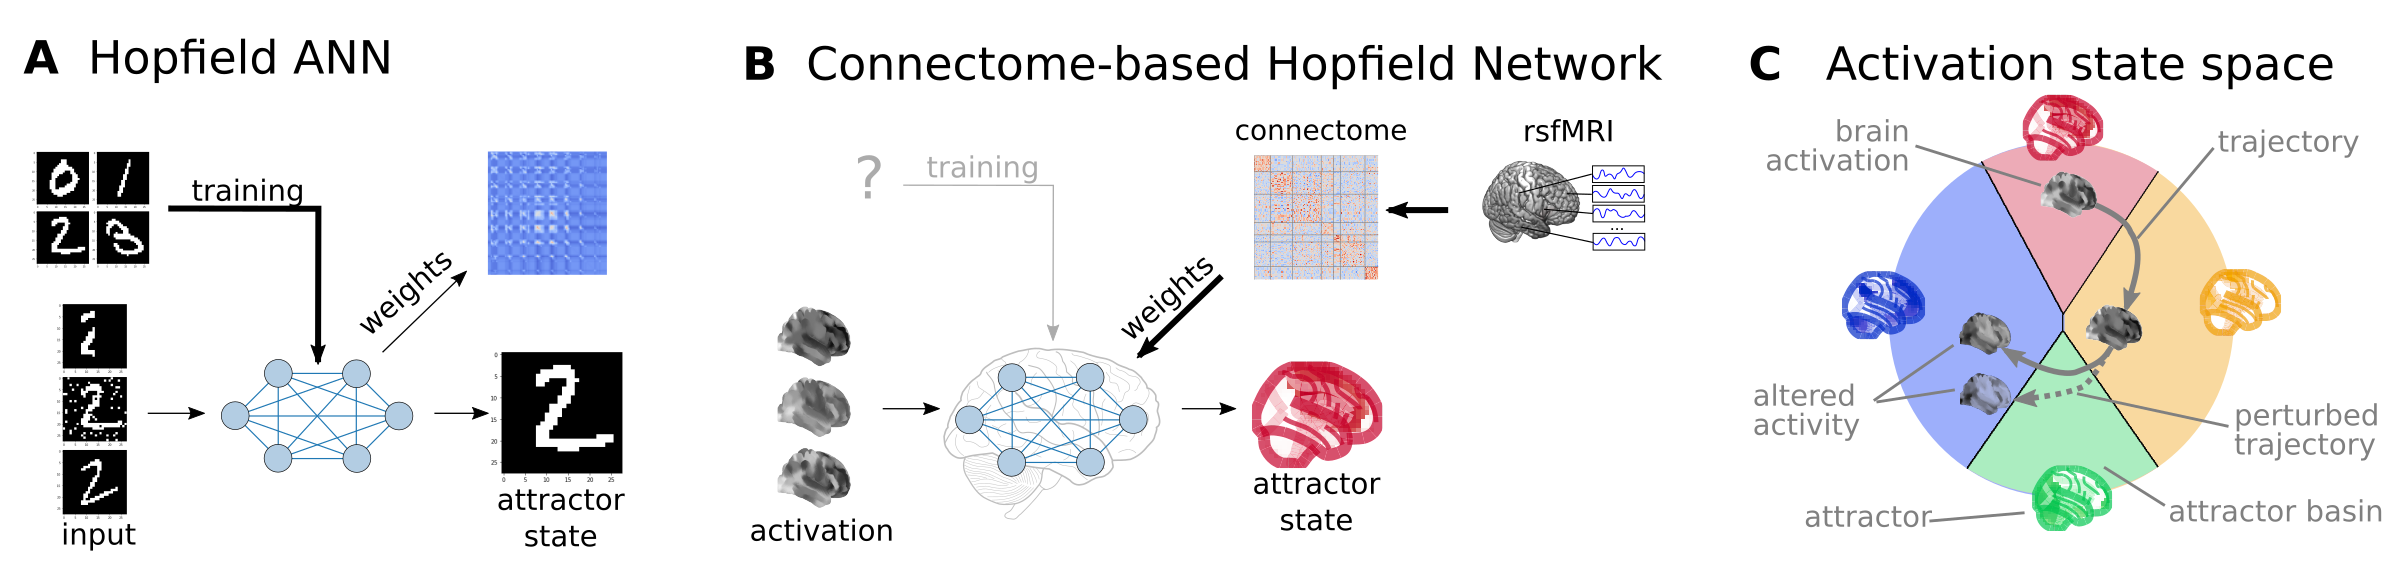
\includegraphics[width=0.7\linewidth]{files/concept-f8eb1650da55952620b72f614e088df3.png}
\caption[]{\textbf{Connectome-based Hopfield networks as models of macro-scale brain dynamics.} \newline
\newline

\textbf{A} Hopfield artificial neural networks (\acrshort{hnn}s)  are a form of recurrent artificial neural networks that serve as content-addressable (``associative'') memory systems. Hopfield networks can be trained to store a finite number of patterns (e.g. via Hebbian learning a.k.a. ``fire together -  wire together''). During the training procedure, the weights of the \acrshort{hnn} are trained so that the stored
patterns become stable attractor states of the network. Thus, when the trained network is presented partial, noisy or corrupted variations of the stored patterns, it can effectively reconstruct the original pattern via an iterative relaxation procedure that converges to the attractor states.
\textbf{B} We consider regions of the brain as nodes of a Hopfield network. Instead of initilaizing the network with the structural wiring of the brain or training it to solve specific tasks, we set its weights empirically, using information about the interregional ``activity flow'' across regions, as estimated via functional brain connectivity. Capitalizing on strong analogies between the relaxation rule of Hopfield networks and the activity flow principle that links activity to connectivity in brain networks, we propose the resulting
functional connectome-based Hopfield neural network (\acrshort{fchnn}) as a minimal phenomenological model for macro-scale brain dynamics.\newline
\textbf{C} The proposed computational framework assigns an energy level, an attractor state and a position in a
low-dimensional embedding to brain activation patterns. Additionally, it models how the entire state-space of viable activation patterns is restricted by the dynamics of the system and how alterations in activity and/or connectivity modify these dynamics.}
\label{concept}
\end{figure}

In the present work, we investigate how well the functional connectome is suited to be an attractor network, map the corresponding attractoir states and model itinerant stochastic dynamics traversing the different basins of attraction of the system.
We use a diverse set of experimental, clinical and meta-analytic studies to evaluate our model's ability to reconstruct various characteristics of resting state brain dynamics, as well as its capacity to detect and explain changes induced by experimental conditions or alterations in brain disorders.

\section{Results}

\subsection{Connectome-based Hopfield network as a model of brain dynamics}

First, we investigated the functional connectome as an attractor network in a sample of n=41 healthy young
participants (Table~\ref{tab-samples}, see Methods Table~\ref{tab-samples} for details). We estimated interregional activity flow \citep{cole2016activity, ito2017cognitive} as the study-level average of regularized partial correlations among the resting state \acrshort{fmri} timeseries of m = 122
functionally defined brain regions (see Methods for details). We then used the standardized functional connectome as the $w_{ij}$  weights of a fully connected recurrent \acrshort{ann}, specifically a continuous-state Hopfield network \citep{hopfield1982neural, koiran1994dynamics}, consisting of $m$ neural units, each having an activity $a_i \in [ -1,1] \subset \mathbb{R})$. Hopfield networks can be initialized by an arbitrary activation pattern (consisting of $m$ activation values) and iteratively updated (i.e. ``relaxed'') until their energy converges a local minimum, that is, to one of the finite number of attractor states (see Methods). The relaxation procedure is based on a simple rule; in each iteration, the activity of a region is constructed as the weighted average of the activities of all other regions, with weights defined by the connectivity between them. The average is then transformed by a sigmoidal activation function, to keep it in the desired [-1,1] interval.
This can be expressed by the following equation:

\begin{equation}
\label{hopfield-update}
{a'}_i = S(\beta \sum_{j=1}^m w_{ij}a_j - b_i)
\end{equation}

where $a'_i$ is the activity of neural unit $i$ in the next iteration and $S(a_j)$ is the sigmoidal activation
function ($S(a) = tanh(a)$ in our implementation) and $b_i$ is the bias of unit $i$ and $\beta$ is the so-called temperature parameter. For the sake of simplicity, we set $b_i=0$ in all our experiments. We refer to this architecture as a functional connectivity-based Hopfield Neural Network (\acrshort{fchnn}).
The relaxation of a \acrshort{fchnn} model can be conceptualized as the repeated application of the activity flow principle \citep{cole2016activity, ito2017cognitive} , simultaneously for all regions: $\dot{a}_i = \sum_{j=1}^m w_{ij}a_j$. The update rule also exhibits analogies with network control theory \citep{gu2015controllability} and the inner workings of neural mass models, as applied e.g. in dynamic causal modeling \citep{daunizeau2012stochastic}.

Hopfield networks assign an energy value to each possible activity configuration \citep{hopfield1982neural, koiran1994dynamics}, which decreases during the relaxation procedure until reaching an equilibrium state with minimal energy (Figure~\ref{attractors}A, top panel).

We used a sufficiently large number of random initializations (n=100000) to obtain all possible attractor states of the connectome-based Hopfield network in study 1 (Figure~\ref{attractors}A, bottom panel).
Consistent with theoretical expectations, we observed that increasing the temperature parameter $\beta$ led to an
increasing number of attractor states (Figure~\ref{attractors}E, left, Figure~\ref{si_att_state_emergence_over_beta}), appearing in symmetric pairs (i.e. $a_i^{(1)} = -a_i^{(2)}$, see Figure~\ref{attractors}G).

\acrshort{fchnn}s, without any modifications, always converge to an equilibrium state.
To incorporate stochastic fluctuations in neuronal activity \citep{robinson2005multiscale}, we introduced weak
Gaussian noise to the \acrshort{fchnn} relaxation procedure. This procedure, referred to as stochastic relaxation, prevents the system from reaching equilibrium and, somewhat similarly to stochastic DCM \citep{daunizeau2012stochastic}, induces complex, heteroclinic system dynamics (Figure~\ref{attractors}B).

In order to enhance interpretability, we obtained the first two principal components (\acrshort{pc}s) of the states sampled from the stochastic relaxation procedure. On the low-dimensional embedding, which we refer to as the \textit{\acrshort{fchnn} projection}, we observed a clear separation of the attractor states (Figure~\ref{attractors}C), with the two symmetric pairs of attractor states located at the extremes of the first and second \acrshort{pc}.
To map the attractors' basins on the space spanned by the first two \acrshort{pc}s (Figure~\ref{attractors}C), we obtained the attractor state of each point visited during the stochastic relaxation and fit a multinomial logistic regression model to predict the attractor state from the first two \acrshort{pc}s.
The resulting model accurately predicted attractor states of arbitrary brain activity patterns, achieving a cross-validated accuracy of 96.5\% (permutation-based p\textless 0.001).
The attractor basins were visualized by using the decision boundaries obtained from this model. (Figure~\ref{attractors}C). We propose the 2-dimensional \acrshort{fchnn} projection depicted on (Figure~\ref{attractors}C) as a simplified representation of brain dynamics, and use it as a basis for all subsequent analyses in this work.

Panel D on Figure~\ref{attractors} uses the \acrshort{fchnn} projection to visualize the conventional Hopfield relaxation procedure. It depicts the trajectory of individual activation maps (sampled randomly from the timeseries data in Study 1) until converging to one of the four attractor states.
Panel E shows that the system does not converge to an attractor state anymore if weak noise is introduced to the system (stochastic relaxation), The resulting path is still influenced by the attractor states' gravity, resulting in a heteroclinic dynamics that resembles the empirical timeseries data (example data on panel F).

\begin{figure}[!htbp]
\centering
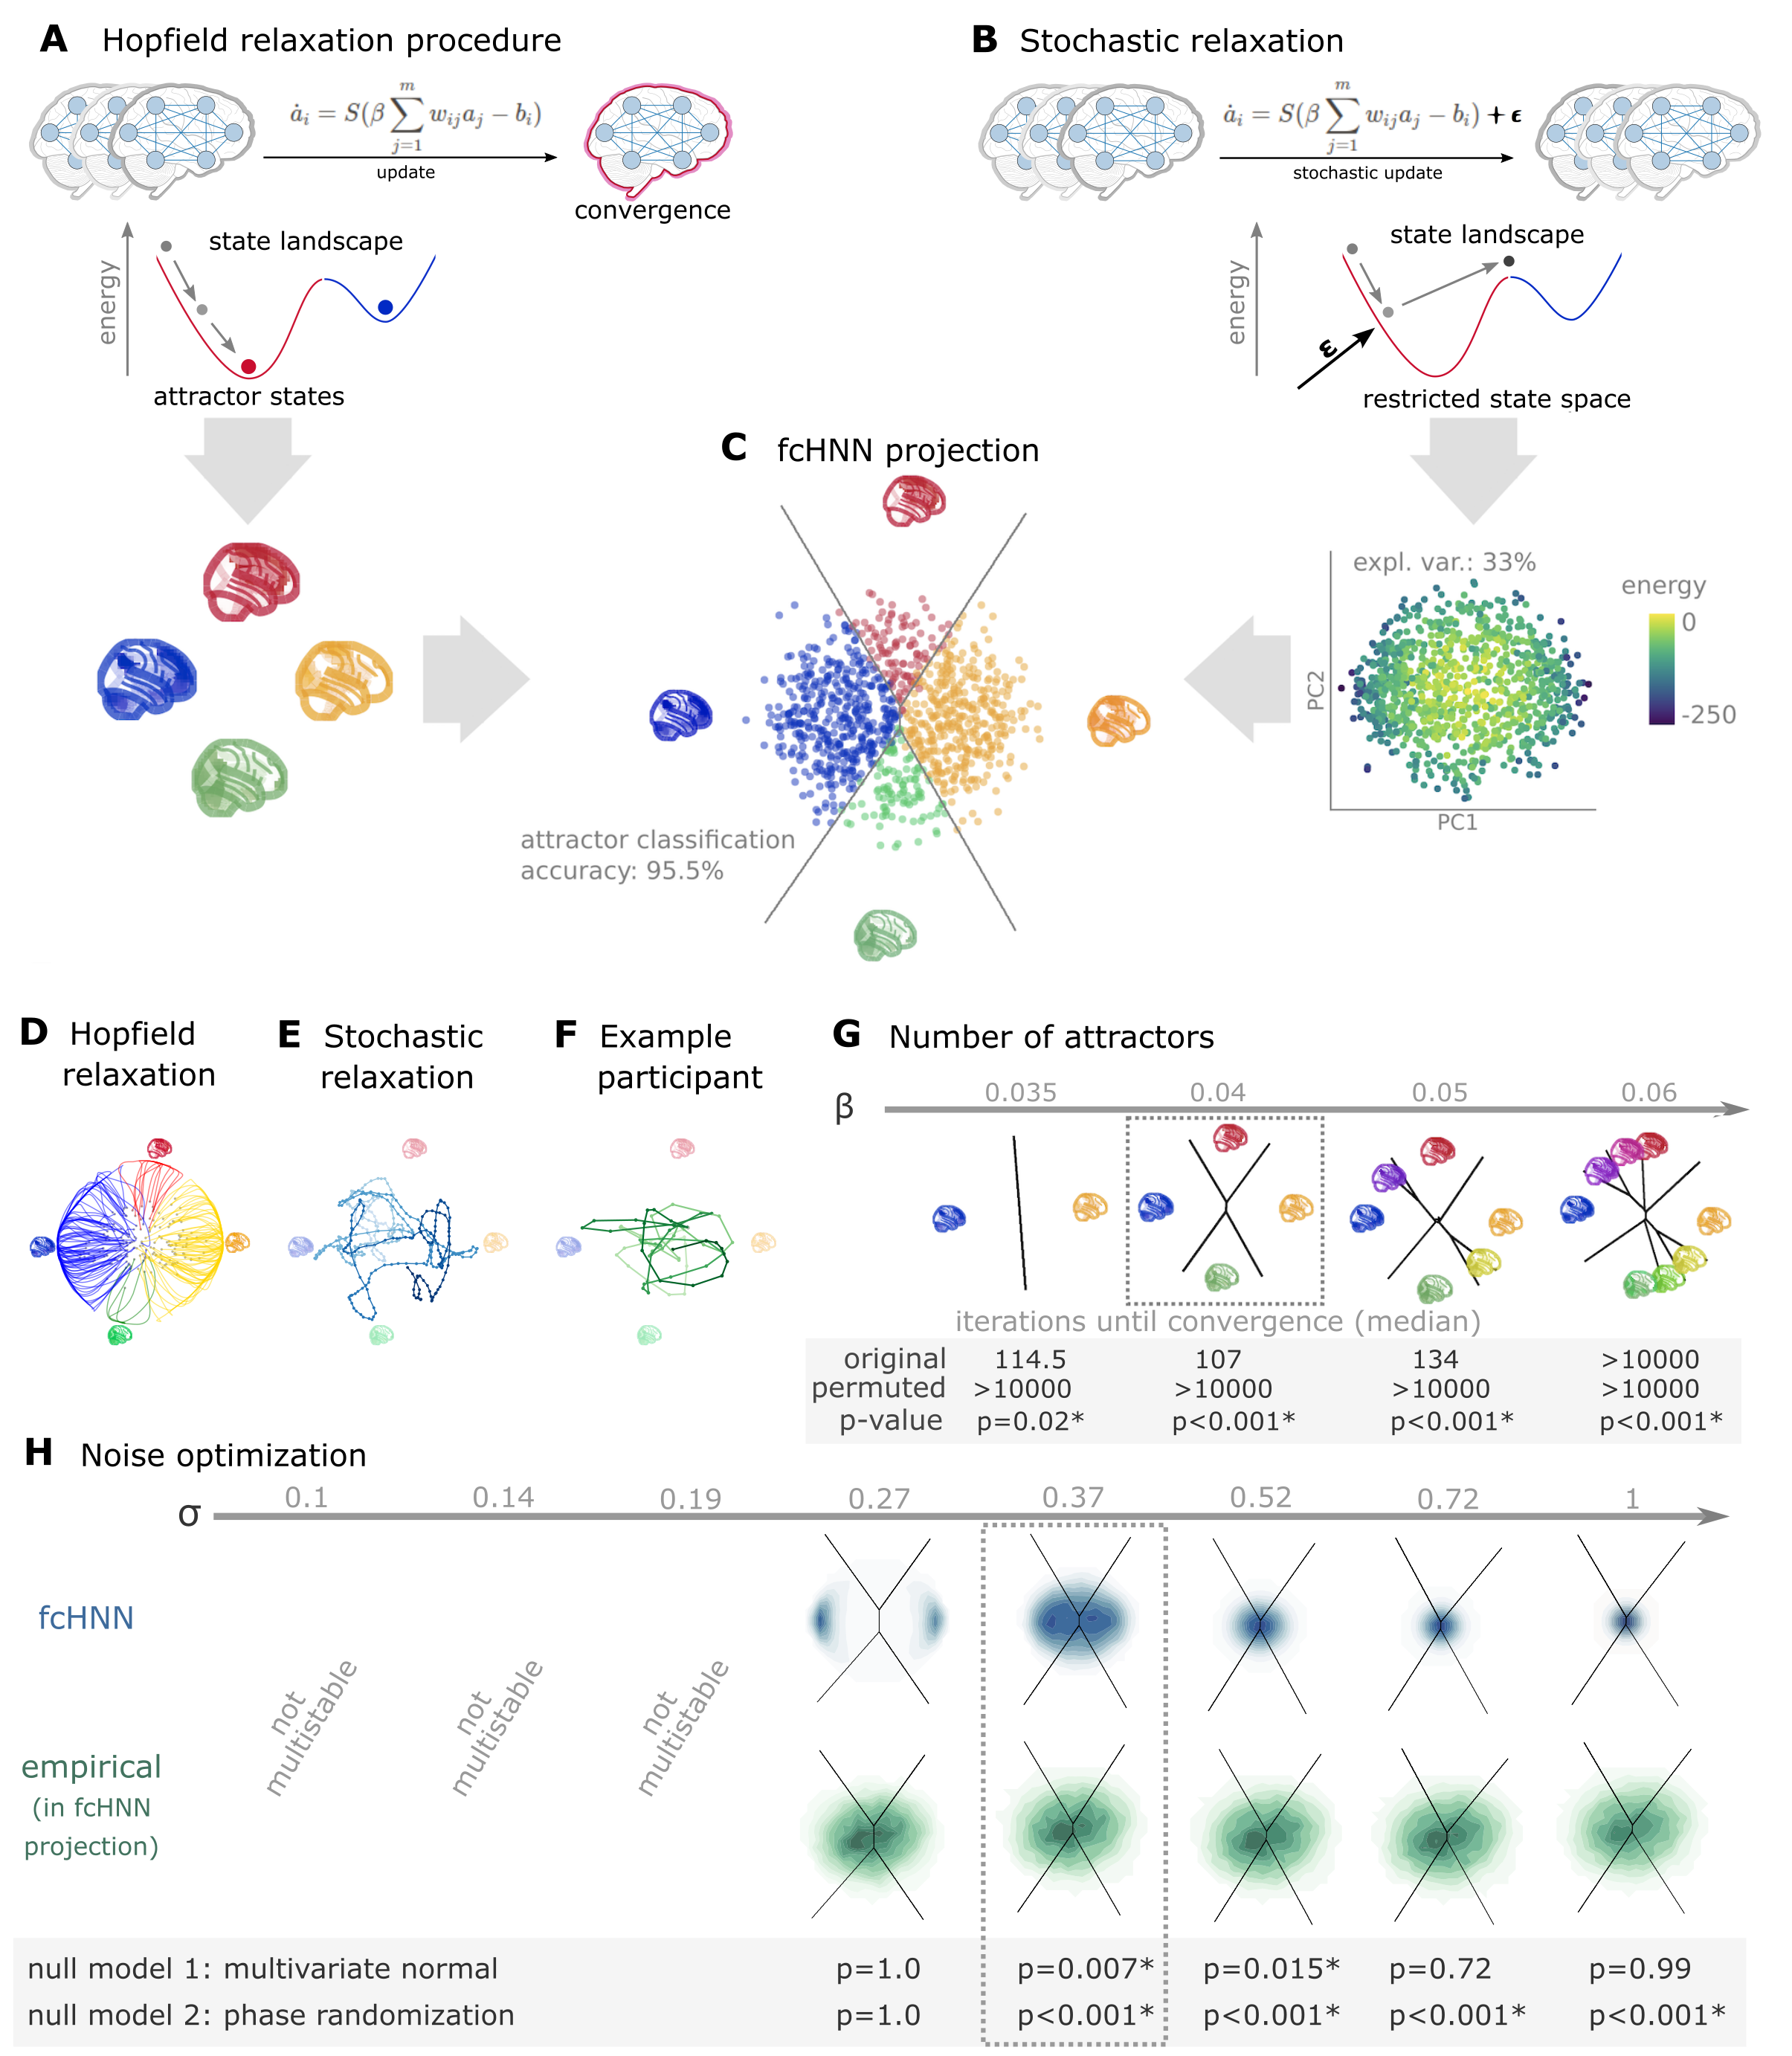
\includegraphics[width=0.7\linewidth]{files/embedding_method-97db4d0c90e864694f03e4f989f47522.png}
\caption[]{\textbf{Attractor states and state-space dynamics of connectome-based Hopfield networks} \newline
\newline

\textbf{A} Top: During so-called relaxation procedure, activities in the nodes of an \acrshort{fchnn} model are iteratively updated based on the activity of all other regions and the connectivity between them. The energy of a
connectome-based Hopfield network decreases during the relaxation procedure until reaching an equilibrium state with
minimal energy, i.e. an attractor state. Bottom: Four attractor states of the \acrshort{fchnn} derived from the
group-level functional connectivity matrix from Table~\ref{tab-samples} (n=44).
\textbf{B} Top: In presence of weak noise (stochastic update), the system
does not converge to equilibrium anymore. Instead, activity traverses on the state landscape in a way
restricted by the topology of the connectome and the ``gravitational pull'' of the attractor states. Bottom: We sample
the ``state landscape'' by running the stochastic relaxation procedure for an extended amount of time (e.g. 100.000 consecutive
stochastic updates), each point representing an activation configuration or state. To construct a
low-dimensional representation of the state space, we take the first two principal components of the simulated activity
patterns. The first two principal components explain approximately 58-85\% of the variance of state energy (depending
on the noise parameter $\sigma$, see Figure~\ref{si_expl_variance_energy}).
\textbf{C} We map all states of the state space sample to their corresponding attractor state, with the conventional
Hopfield relaxation procedure (A). The four attractor states are also visualized in their corresponding position on the
\acrshort{pc}A-based projection. The first two principal components yield a clear separation of the attractive state basins
(cross-validated classification accuracy: 95.5\%, Figure~\ref{si_classification_acc_state_basins}). We refer to the resulting visualization
as the \acrshort{fchnn} projection and use it to visualize \acrshort{fchnn}-derived and empirical brain dynamics throughout the rest of
the manuscript.
\textbf{D} The \acrshort{fchnn} of study 1 seeded with real activation maps (gray dots) of an example participant. All activation maps converge to one of the four attractor states during the relaxation procedure (without noise) and the system reaches equilibrium. Trajectories are colored by attractor state.
\textbf{E} Illustration of the stochastic relaxation procedure in the same \acrshort{fchnn} model, seeded from a single starting point (activation pattern). The system does not converge to an attractor state but instead traverses the state space in a way restricted by the topology of the connectome and the ``gravitational pull'' of the attractor states. The shade of the trajectory changes with increasing number of iterations. The trajectory is smoothed with a moving average over 10 iterations for visualization purposes.
\textbf{F} Real resting state \acrshort{fmri} data of an example participant from study 1, plotted on the \acrshort{fchnn} projection. The shade of the trajectory changes with an increasing number of iterations. The trajectory is smoothed with a moving average over 10 iterations for visualization purposes.
\textbf{G} Consistent with theoretical expectations, we observed that increasing the temperature parameter $\beta$ led to an
increasing number of attractor states, emerging in a nested fashion (i.e. the basin of a new attractor state is fully contained within the basin of a previous one). When contrasting the functional connectome-based \acrshort{hnn} with a null model based on symmetry-retaining permuted variations of the connectome, we found that the topology of the original (unpermuted) functional brain connectome makes it significantly better suited to function as an attractor network; than the permuted null model. Table contains the meadian number of iterations until convergence for the original and permuted connectomes for different temperature parameters $\beta$ and the corresponding p-value.
\textbf{H} We optimized the noise parameter $\sigma$ of the stochastic relaxation procedure for 8 different $\sigma$ values over a logarithmic range between $\sigma=0.1$ and 1 so that the similarity (the timeframes distribution over the attractor basins) is maximized between the empirical data and the \acrshort{fchnn}-generated data. We used to null models to assess the significance of similarity: one based on multivariate normal data, with the covariance matrix set to the functional connectome's covariance matrix, and one based on spatial phase-randomization. P-values are given in the table at the bottom of the panel. The \acrshort{fchnn} only reached multistability with $\sigma>0.19$, and it provided the most accurate reconstruction of the real data with $\sigma=0.37$ (p=0.007, and p\textless 0.001 for the two null models).}
\label{attractors}
\end{figure}

In study 1, we have investigated the convergence process of the functional connectivity-based \acrshort{hnn} and contrasted it with a null model based on permuted variations of the connectome (while retaining the symmetry of the matrix). This null model preserves the sparseness and the degree distribution of the connectome, but destroys its topological structure (e.g. clusteredness). We found that the topology of the original (unpermuted) functional brain connectome makes it significantly better suited to function as an attractor network; than the permuted null model.
While the original connectome based \acrshort{hnn} converged to an attractor state in less than 150 iterations in more than 50\% of the cases, the null model did not reach convergence in more than 98\% of the cases, even after 10000 iterations (Figure~\ref{attractors}G, Figure~\ref{si_convergence}). This result was robustly observed, independent of the temperature parameter beta.
We set the temperature parameter for the rest of the paper to a value providing the fastest convergence ($\beta=0.4$, median iterations: 107), resulting in 4 distinct attractor states. The primary motivation for selecting $\beta=0.4$ was to reduce computational burden for further analyses. However, as with increasing temperature, attractor states emerge in a nested fashion (i.e. the basin of a new attractor state is fully contained within the basin of a previous one), we expect that the results of the following analyses would be, although more detailed, but qualitatively similar with higher $\beta$ values.

We optimized the noise parameter $\sigma$ of the stochastic relaxation procedure for 8 different $\sigma$ values over a logarithmic range between $\sigma=0.1$ and 1 so that the similarity (the timeframes distribution over the attractor basins) is maximized between the empirical data and the \acrshort{fchnn}-generated data. We contrasted this similarity with two null-models (Figure~\ref{attractors}H). First we generated null-data as random draws from a multivariate normal distribution with co-variance matrix set to the functional connectome's covariance matrix (partial correlation-based connectivity estimates). This serves as a baseline for generating data that optimally matches the empirical data in terms of distribution and spatial autocorrelation, as based on information on the underlying co-variance structure (and given Gaussian assumptions), but without any mechanistic model of the generative process, e.g. without modelling any non-linear and non-Gaussian effects and temporal autocorrelations stemming from recurrent activity flow). We found that The \acrshort{fchnn} only reached multistability with $\sigma>0.19$, and it provided more accurate reconstruction of the real data than the null model for $\sigma=0.37 and \sigma=0.52$ (p=0.007 and 0.015, $\chi^2 dissimilarity:$11.16$and 21.57$, respectively).
With our second null model, we investigated whether the \acrshort{fchnn}-reconstructed data is more similar to the empirical data than synthetic data with identical distribution and spatial autocorrelation structure (generated by spatial phase randomization of the original volumes, see Methods).
We found that the \acrshort{fchnn}s significantly outperform this null model with all investigated $\sigma$ values if $\sigma \geq 0.37 (p<0.001 for all)$
Based on this coarse optimization procedure, we set $\sigma=0.37$ for all subsequent analyses.

\subsection{Reconstruction of resting state brain dynamics}

The spatial patterns of the obtained attractor states exhibit high neuroscientific relevance and closely resemble previously described large-scale brain systems. (Figure~\ref{rest-validity}A).

The first pair of attractors (mapped on \acrshort{pc}1, horizontal axis) represent two complementary brain systems, that have been previously found in anatomical, functional, developmental, and evolutionary hierarchies, as well as gene expression, metabolism, and blood flow, (see \cite{sydnor2021neurodevelopment} for a review), an reported under various names, like intrinsic and extrinsic systems \citep{golland2008data}, Visual-Sensorimotor-Auditory and Parieto-Temporo-Frontal ``rings'' \citep{cioli2014differences}, ``primary'' brain states \citep{chen2018human}, unimodal-to-transmodal principal gradient \citep{margulies2016situating, huntenburg2018large} or sensorimotor-association axis \citep{sydnor2021neurodevelopment}.
A common interpretation of these two patterns is that they represent (i) an ``extrinsic'' system linked to the immediate sensory environment and (ii) an ``intrinsic'' system for higher-level internal context, commonly referred to as the default mode network \citep{raichle2001default}.
A common interpretation of these two patterns is that they represent (i) an ``extrinsic'' system linked to the immediate sensory environment and (ii) an ``intrinsic'' system for higher-level internal context, commonly observed during resting states.
The other pair of attractors spans an orthogonal axis, and resemble to patterns commonly associated with perception--action cycles \citep{fuster2004upper}, and described as a gradient across sensory-motor modalities \citep{huntenburg2018large}, recruiting regions associated with active inference (e.g. motor cortices) and perceptual inference (e.g visual areas).

\begin{figure}[!htbp]
\centering
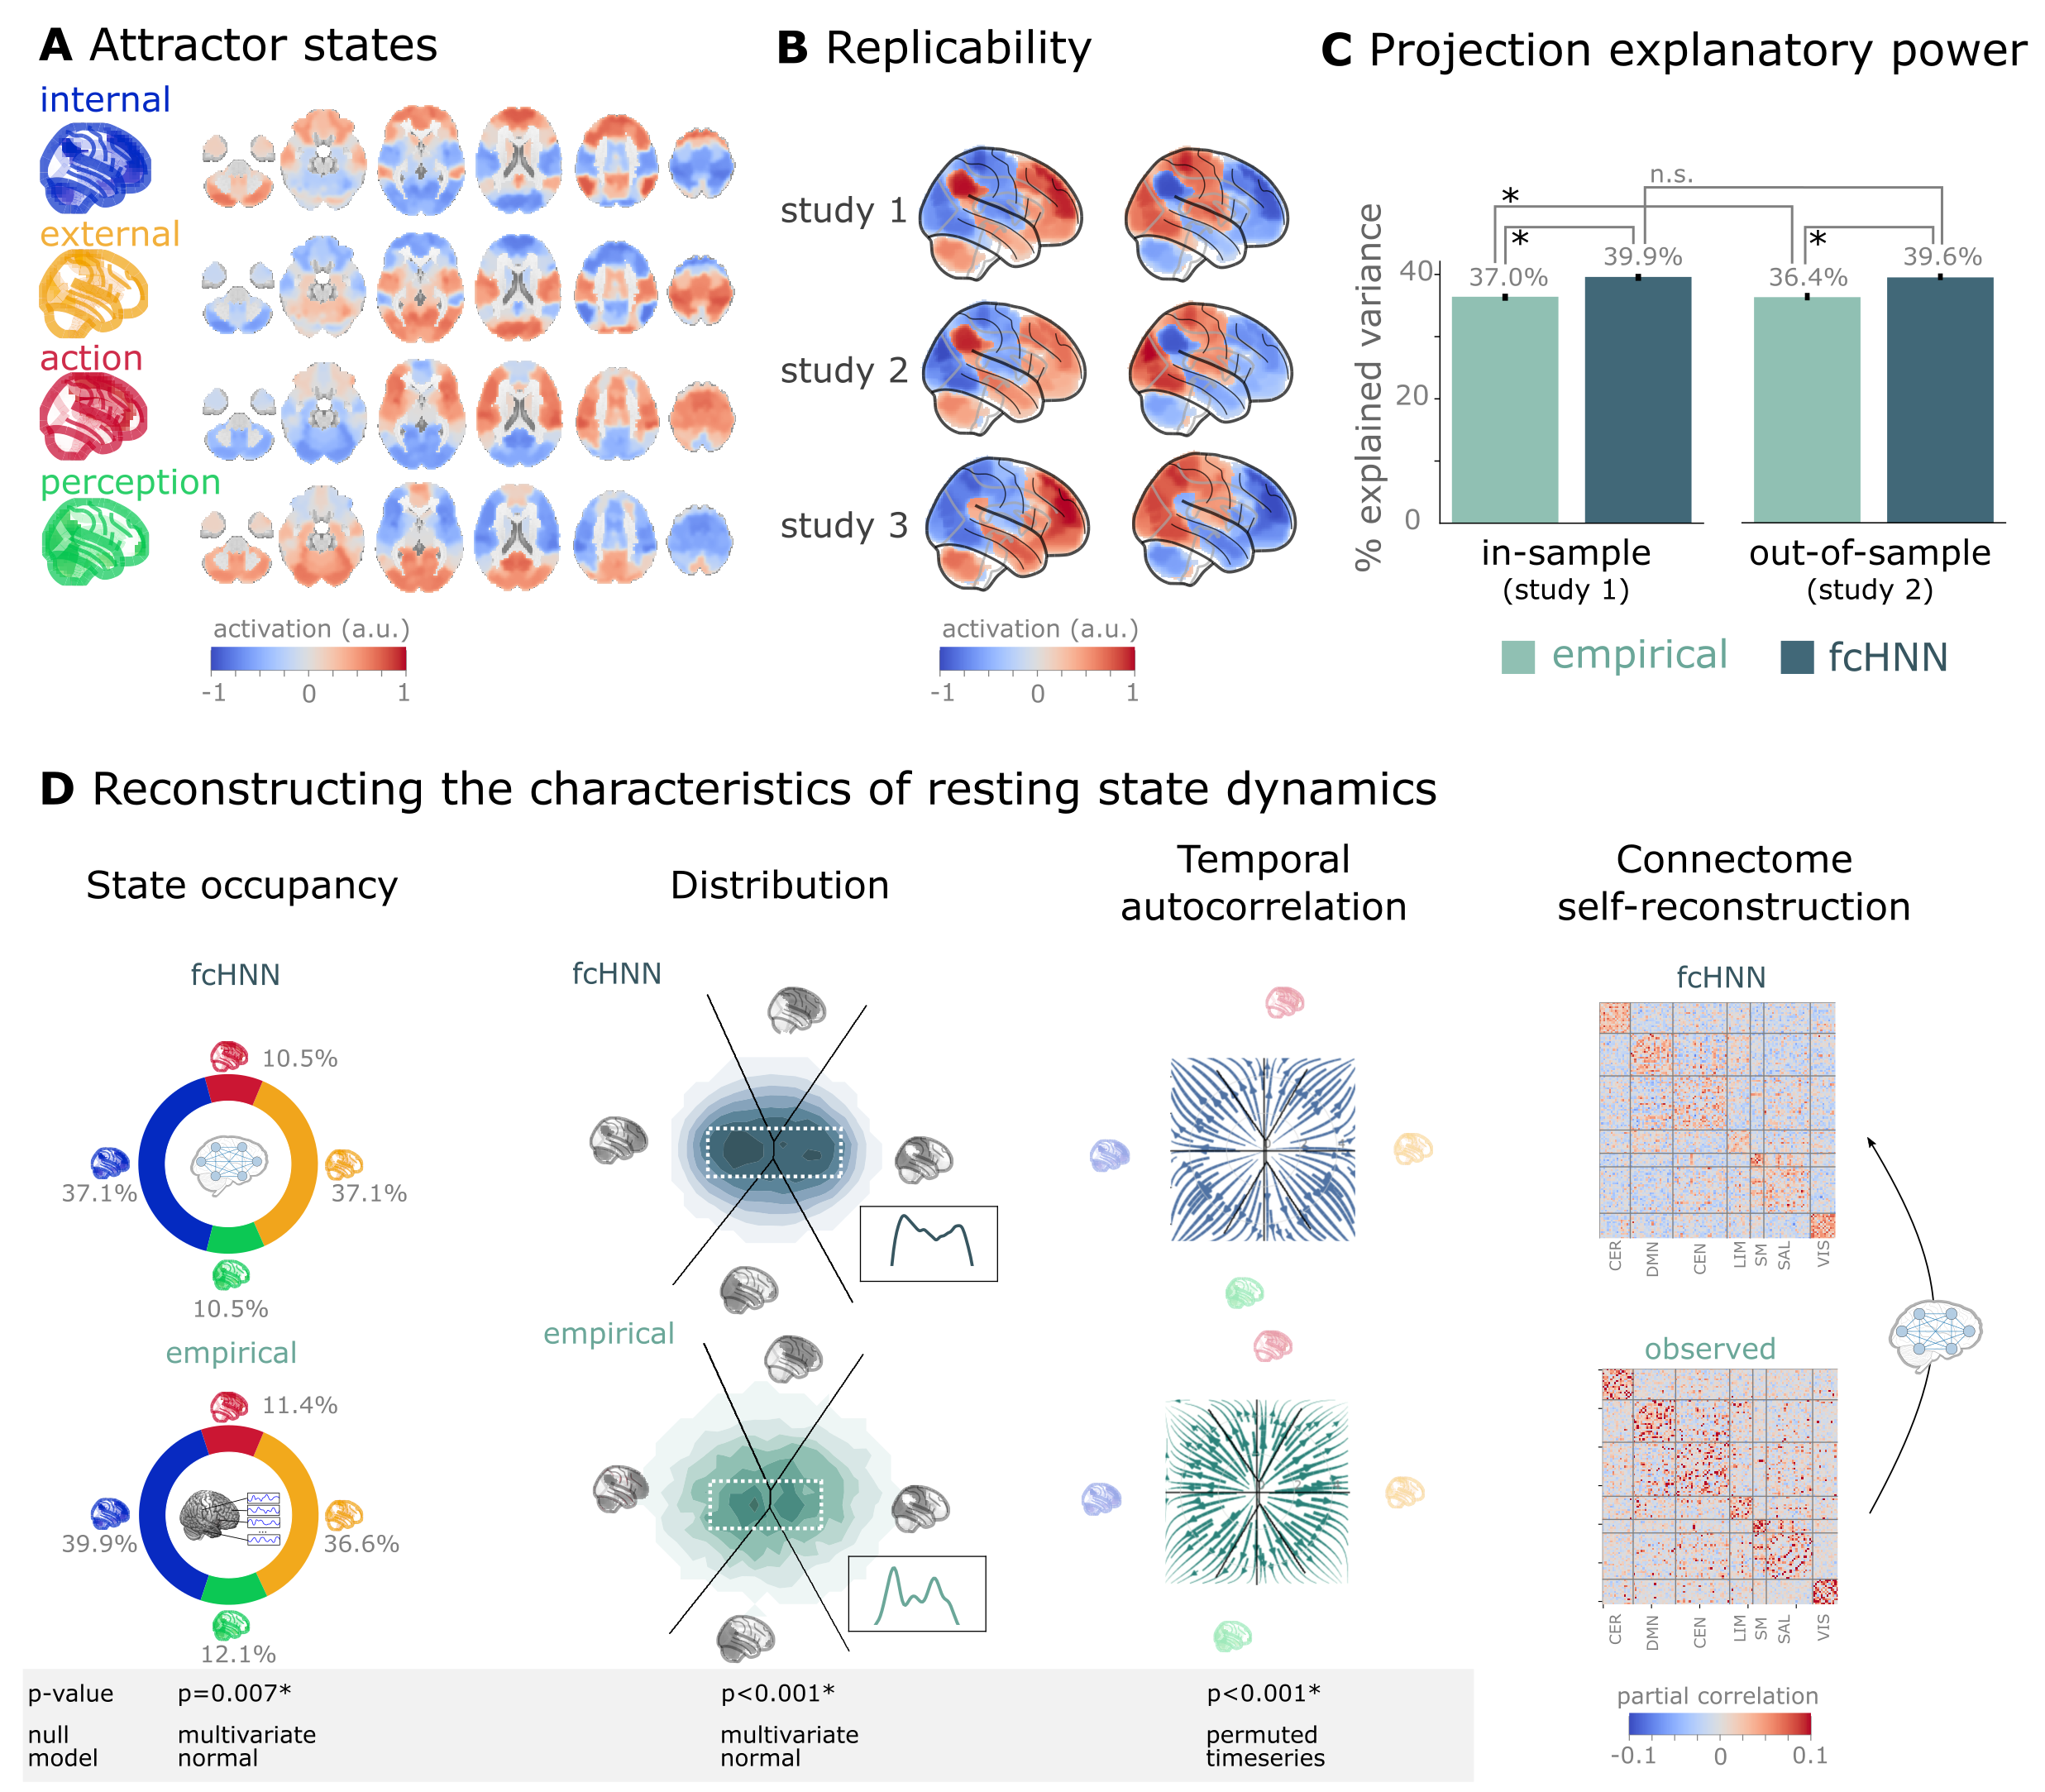
\includegraphics[width=0.7\linewidth]{files/face_validity-ec95f8d876dc74298f5d8f0d8d7cb8f2.png}
\caption[]{\textbf{Connectome-based Hopfield networks reconstruct characteristics of real resting state brain activity.}\newline
\newline

\textbf{A} The four attractor states of the \acrshort{fchnn} model from study 1 reflect brain activation
patterns with high neuroscientific relevance, representing sub-systems previously associated with ``internal context''
(blue), ``external context'' (yellow), ``action'' (red) and ``perception'' (green)
\citep{golland2008data, cioli2014differences, chen2018human, fuster2004upper, margulies2016situating}.
\textbf{B} The attractor states show excellent replicability in two external datasets (study 2 and 3, mean correlation 0.93).
\textbf{C} The \acrshort{fchnn} projection (first two \acrshort{pc}s of the \acrshort{fchnn} state space) explains significantly more variance (p\textless 0.0001) in the real
resting state \acrshort{fmri} data than principal components derived from the real resting state data itself and generalizes
better (p\textless 0.0001) to out-of-sample data (study 2). Error bars denote 99\% bootstrapped confidence intervals.
\textbf{D} The \acrshort{fchnn} analysis reliably predicts various characteristics of real resting state \acrshort{fmri} data, such as the fraction of time spent on the basis of the four attractors (first column, p=0.007, contrasted to the multivariate normal null model), the distribution of the data on the \acrshort{fchnn}-projection (second column, p\textless 0.001, contrasted to the multivariate normal null model) and the temporal autocorrelation structure of the real data (third column, p\textless 0.001, contrasted to a null model based on temporally permuted data). This analysis was based on flow maps of the mean trajectories (i.e. the characteristic timeframe-to-timeframe transition direction) in \acrshort{fchnn}-generated data, as compared to a shuffled null model representing zero temporal autocorrelation. For more details, see Methods. Furthermore, (rightmost column), stochastic \acrshort{fchnn}s are capable of self-reconstruction: the timeseries resulting from the stochastic relaxation procedure mirror the co-variance structure of the functional connectome the \acrshort{fchnn} model was initialized with. While the self-reconstruction probability in itself does not strengthen the face-validity of the approach (no unknown information is reconstructed), it is a strong indicator of the model's construct validity; i.e. that systems that behave like the proposed model inevitably ``leak'' their weights into the activity time series.}
\label{rest-validity}
\end{figure}

The discovered attractor states demonstrate remarkable replicability (mean Pearson's correlation 0.93) across the discovery dataset (study 1) and two independent replication datasets (Table~\ref{tab-samples}, Figure~\ref{rest-validity}C). Moreover, they were found to be significantly more robust to noise added to the connectome than nodal strengths scores (used as a reference, see Figure~\ref{si_noise_robustness_weights} for details).

Further analysis in study 1 showed that connectome-based Hopfield models accurately reconstructed multiple characteristics of true resting-state data.
First, the two axes (first two \acrshort{pc}s) of the \acrshort{fchnn} projection accounted for a substantial amount of variance in the real resting-state \acrshort{fmri} data in study 1 (mean $R^2=0.399$) and generalized well to out-of-sample data (study 2, mean $R^2=0.396$)  (Figure~\ref{rest-validity}E). The explained variance of the \acrshort{fchnn} projection significantly exceeded that of the first two \acrshort{pc}s derived directly from the real resting-state \acrshort{fmri} data itself ($R^2=0.37$ and 0.364 for in- and out-of-sample analyses).

Second, \acrshort{fchnn} analyses accurately reconstructed various aspects of true resting state brain dynamics.
During stochastic relaxation, the \acrshort{fchnn} model was found to spend approximately three-quarters of the time on the basis of the first two attractor states and one-quarter on the basis of the second pair of attractor states (approximately equally distributed between pairs). We observed similar temporal occupancies in the real data Figure~\ref{rest-validity}D left column), statistically significant with two different null models (Figure~\ref{si_state_occupancy_null_models}). Fine-grained details of the bimodal distribution observed in the real resting-state \acrshort{fmri} data were also convincingly reproduced by the \acrshort{fchnn} model (Figure~\ref{rest-validity}F and Figure~\ref{attractors}D, second column).
Not only spatial activity patterns but also timeseries generated by the fchNN are similar to empirical timeseries data. Next to the visual similarity shown on Figure~\ref{attractors}E and F, we observed a statistically significant similarity between the average trajectories of \acrshort{fchnn}-generated and real timeseries ``flow'' (i.e. the characteristic timeframe-to-timeframe transition direction), as compared to null-models of zero temporal autocorrelation (randomized timeframe order, Figure~\ref{rest-validity}D, third column Methods for analysis details).
Finally, \acrshort{fchnn}s were found to generate signal that preserves the covariance structure of the real functional connectome, indicating that dynamic systems of this type (including the brain) inevitably ``leak'' their underlying structure into the activity time series, strengthening the construct validity of our approach (Figure~\ref{rest-validity}D).

\subsection{An explanatory framework for task-based brain activity}

Next to reproducing various characteristics of spontaneous brain dynamics, \acrshort{fchnn}s can also be used to model responses to various perturbations. We obtained task-based \acrshort{fmri} data from a study by \citet{woo2015distinct} (Table~\ref{tab-samples}, n=33, see Figure~\ref{rest-validity}), investigating the neural correlates of pain and its self-regulation.

We found that activity changes due to pain (taking into account hemodynamics, see Methods) were characterized on the \acrshort{fchnn} projection by a shift towards the attractor state of action/execution (permutation test for mean projection difference by randomly swapping conditions, p\textless 0.001, Figure~\ref{task-validity}A, left). Energies, as defined by the \acrshort{fchnn}, were also significantly different between the two conditions (p\textless 0.001), with higher energies during pain stimulation.

When participants were instructed to up- or downregulate their pain sensation (resulting in increased and decreased pain reports and differential brain activity in the nucleus accumbens, NAc (see \cite{woo2015distinct} for details), we observed further changes of the location of momentary brain activity patterns on the \acrshort{fchnn} projection (p\textless 0.001, Figure~\ref{task-validity}A, right), with downregulation pulling brain dynamics towards the attractor state of internal context and perception. Interestingly, self-regulation did not trigger significant energy changes (p=0.36).

\begin{figure}[!htbp]
\centering
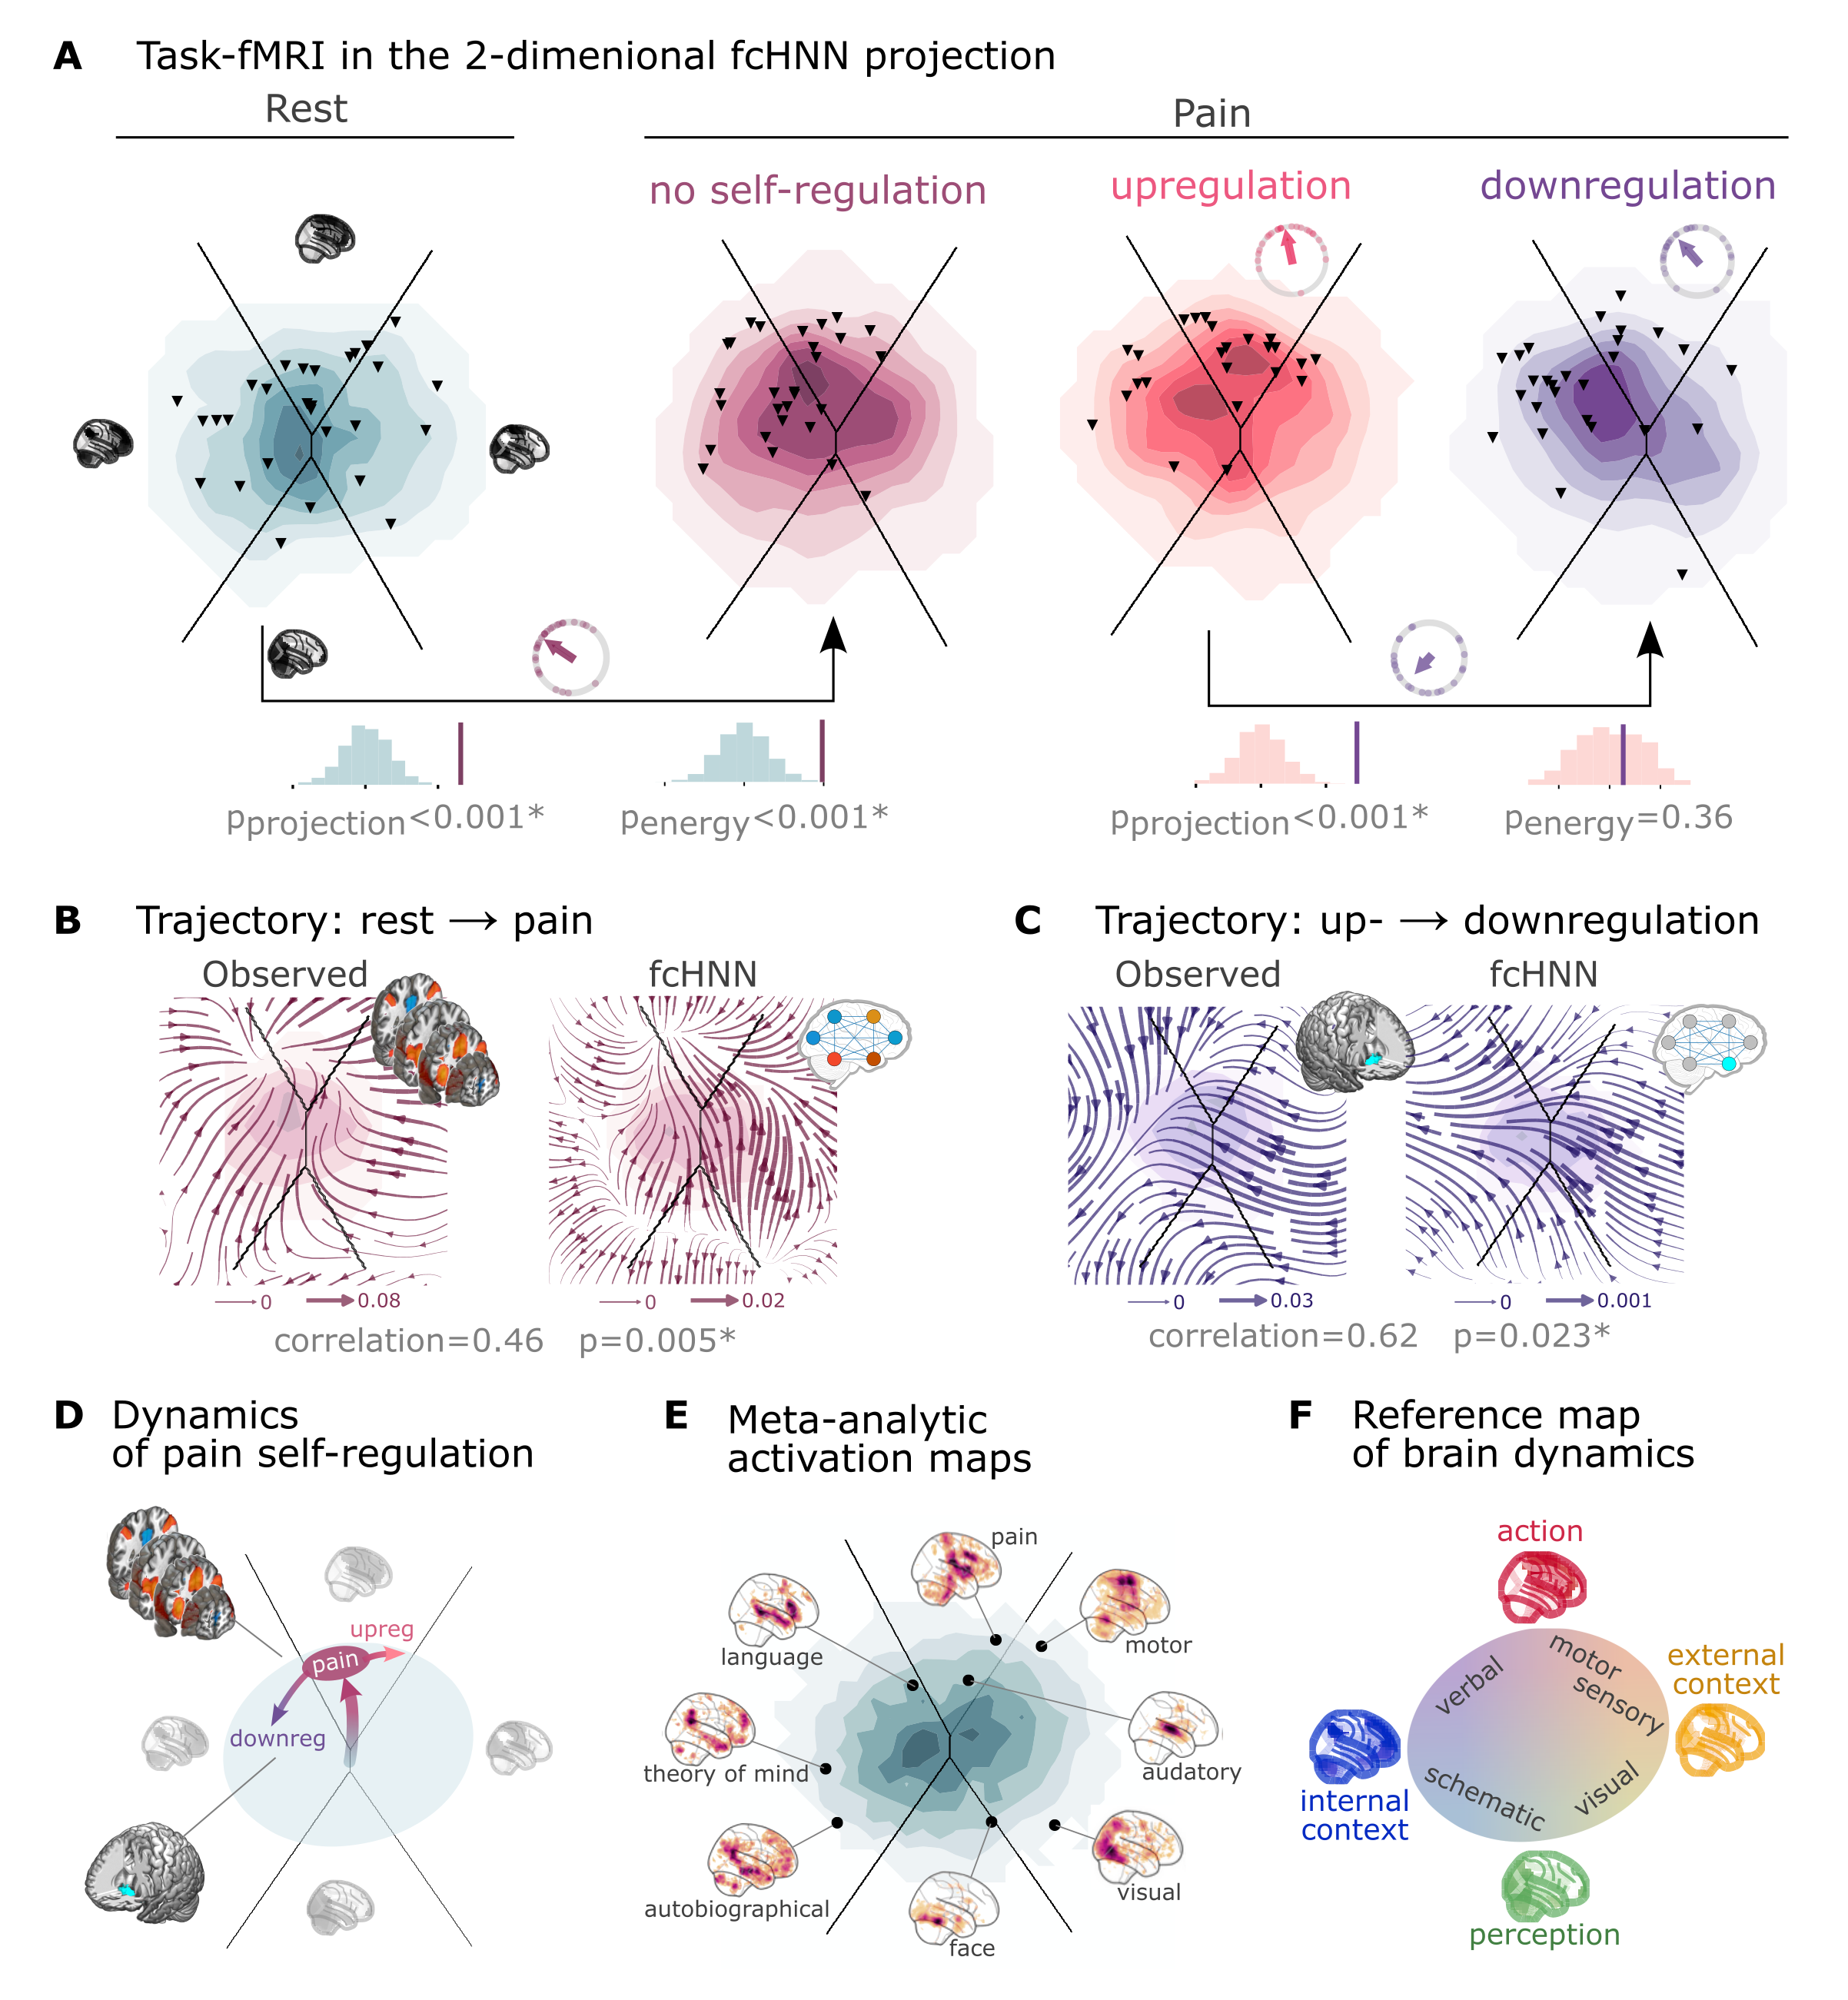
\includegraphics[width=0.7\linewidth]{files/task_validity-5c6ee7fab5b50ac29504e3eb9e837693.png}
\caption[]{\textbf{Empirical Hopfield-networks reconstruct real task-based brain activity.} \newline

\textbf{A} Functional MRI time-frames during pain stimulation from Table~\ref{tab-samples} (second \acrshort{fchnn} projection plot)
and self-regulation (third and fourth) are distributed differently on the \acrshort{fchnn} projection than brain states
during rest (first projection, permutation test, p\textless 0.001 for all). Energies, as defined by the Hopfield model, are also
significantly different between rest and the pain conditions (permutation test, p\textless 0.001), with higher energies during
pain stimulation. Triangles denote participant-level mean activations in the various blocks (corrected for
hemodynamics). Small circle plots show the directions of the change for each individual (points) as well as the mean direction
across participants (arrow), as compared to the reference state (downregulation for the last circle plot, rest for all
other circle plots).
\textbf{B} Flow-analysis (difference in the average timeframe-to-timeframe transition direction) reveals a non-linear difference in brain dynamics during pain and rest (left). When introducing weak pain-related signal in the \acrshort{fchnn} model during stochastic relaxation, it accurately reproduces these non-linear flow differences (right).
\textbf{C} Simulating activity in the Nucleus Accumbens (NAc) (the region showing significant activity differences in \cite{woo2015distinct}) reconstructs the observed non-linear flow difference between up- and downregulation (left).
\textbf{D} Schematic representation of brain dynamics during pain and its up- and downregulation, visualized on the \acrshort{fchnn}  projection. In the proposed framework, pain does not simply elicit a direct response in certain regions, but instead, shifts spontaneous brain dynamics towards the ``action'' attractor, converging to a characteristic ``ghost attractor'' of pain. Down-regulation by NAc activation exerts force towards the attractor of internal context, leading to the brain less frequent ``visiting'' pain-associated states.
\textbf{E} Visualizing meta-analytic activation maps (see Table~\ref{si-tab-neurosynth} for details) on the \acrshort{fchnn} projection captures intimate relations between the corresponding tasks and \textbf{F} serves as a basis for a \acrshort{fchnn}-based theoretical interpretative framework for spontaneous and task-based brain dynamics. In the proposed framework, task-based activity is not a mere response to external stimuli in certain brain locations but a perturbation of the brain's characteristic dynamic trajectories, constrained by the underlying functional connectivity. From this perspective, ``activity maps'' from conventional task-based \acrshort{fmri} analyses capture time-averaged differences in these whole brain dynamics.}
\label{task-validity}
\end{figure}

Next, we conducted a ``flow analysis'' on the \acrshort{fchnn} projection, quantifying how the average timeframe-to-timeframe transition direction differs on the \acrshort{fchnn} projection between conditions (see Methods).
This analysis unveiled that during pain (Figure~\ref{task-validity}B, left side), brain activity tends to gravitate towards a distinct point on the projection on the boundary the basins of the internal and action attractors, which we term the ``ghost attractor'' of pain (similar to \cite{vohryzek2020ghost}). In case of downregulation (as compared to upregulation), brain activity is pulled away from the pain-related ``ghost attractor'' (Figure~\ref{task-validity}C, left side), towards the attractor of internal context.

Our \acrshort{fchnn} was able to accurately reconstruct these non-linear dynamics by adding a small amount of realistic ``control signal'' (similarly to network control theory \citet{liu2011controllability, gu2015controllability}). To simulate the alterations in brain dynamics during pain stimulation, we acquired a meta-analytic pain activation map \citep{zunhammer2021meta} (n=603) and incorporated it as a control signal added to each iteration of the stochastic relaxation procedure. The ghost attractor found in the empirical data was present across a relatively wide range of signal-to-noise (SNR) values (Figure~\ref{si_pain_ghost_attractor_sim}). Results with SNR=0.005 are presented on Figure~\ref{task-validity}B, right side (Pearson's r = 0.46, p=0.005 based on randomizing conditions on a per-participant basis).

The same model was also able to reconstruct the observed non-linear differences in brain dynamics between the up- and downregulation conditions (Pearson's r = 0.62, p=0.023) without any further optimization (SNR=0.005,
Figure~\ref{task-validity}C, right side). The only change we made to the model was the addition (downregulation) or
subtraction (upregulation) of control signal in the NAc (the region in which \citep{woo2015distinct} observed significant changes between up- and downregulation), introducing a signal difference of $\Delta$SNR=0.005 (the same value we found optimal in the pain-analysis). Results were reproducible with lower NAc SNRs, too (Figure~\ref{si_downreg_trajectory_sim}).

To provide a comprehensive picture on how tasks and stimuli other than pain map onto the \acrshort{fchnn} projection, we obtained various task-based meta-analytic activation maps from Neurosynth (see Methods) and plotted them on the \acrshort{fchnn} projection (Figure~\ref{task-validity}E). This analysis reinforced and extended our interpretation of the four investigated attractor states and shed more light on how various functions are mapped on the axes of internal vs. external context and perception vs. action.
In the coordinate system of the \acrshort{fchnn} projection, visual processing is labeled ``external-perception'', sensory-motor processes fall into the ``external-active'' domain, language, verbal cognition and working memory belongs to the ``internal-active'' region and long-term memory as well as social and autobiographic schemata fall into the ``internal-perception'' regime (Figure~\ref{task-validity}F).

\subsection{Clinical relevance}

We obtained data from n=172 autism spectrum disorder (\acrshort{asd}) and typically developing control (TDC) individuals, acquired at the New York University Langone Medical Center, New York, NY, USA (NYU) and generously shared in the Autism Brain Imaging Data Exchange dataset (Table~\ref{tab-samples}: \acrshort{abide}, \citep{di2014autism}.
After excluding high-motion cases (with the same approach as in Study 1-4, see Methods), we visualized the distribution of time-frames on the \acrshort{fchnn}-projection separately for the \acrshort{asd} and TDC groups (Figure~\ref{clinical-validity}A).
First, we assigned all timeframes to one of the 4 attractor states with the \acrshort{fchnn} from study 1 and found several significant differences in the mean activity on the attractor basins (see Methods) of the \acrshort{asd} group as compared to the respective controls (Figure~\ref{clinical-validity}B).
Strongest differences were found on the ``action-perception'' axis (Table~\ref{tab-clinical-results}), with increased activity of the sensory-motor and mid\acrshort{dl}e cingular cortices during ``action-execution'' related states and increased visual and decreased sensory and auditory activity during ``perception'' states, likely reflecting the widely acknowledged, yet poorly understood, perceptual atypicalities in \acrshort{asd} \citep{hadad2019perception}. \acrshort{asd} related changes in the internal-external axis were characterized by more involvement of the posterior cingulate, the precuneus, the nucleus accumbens, the dorsolateral prefrontal cortex (\acrshort{dl}\acrshort{pfc}), the cerebellum (Crus II, lobule VII) and inferior temporal regions during activity of the internalizing subsystem (Table~\ref{tab-clinical-results}). While similar, default mode network (DMN)-related changes have often been attributed to an atypical integration of information about the ``self'' and the ``other'' \citep{padmanabhan2017default}, a more detailed \acrshort{fchnn}-analysis may help to further disentangle the specific nature of these changes.

\begin{figure}[!htbp]
\centering
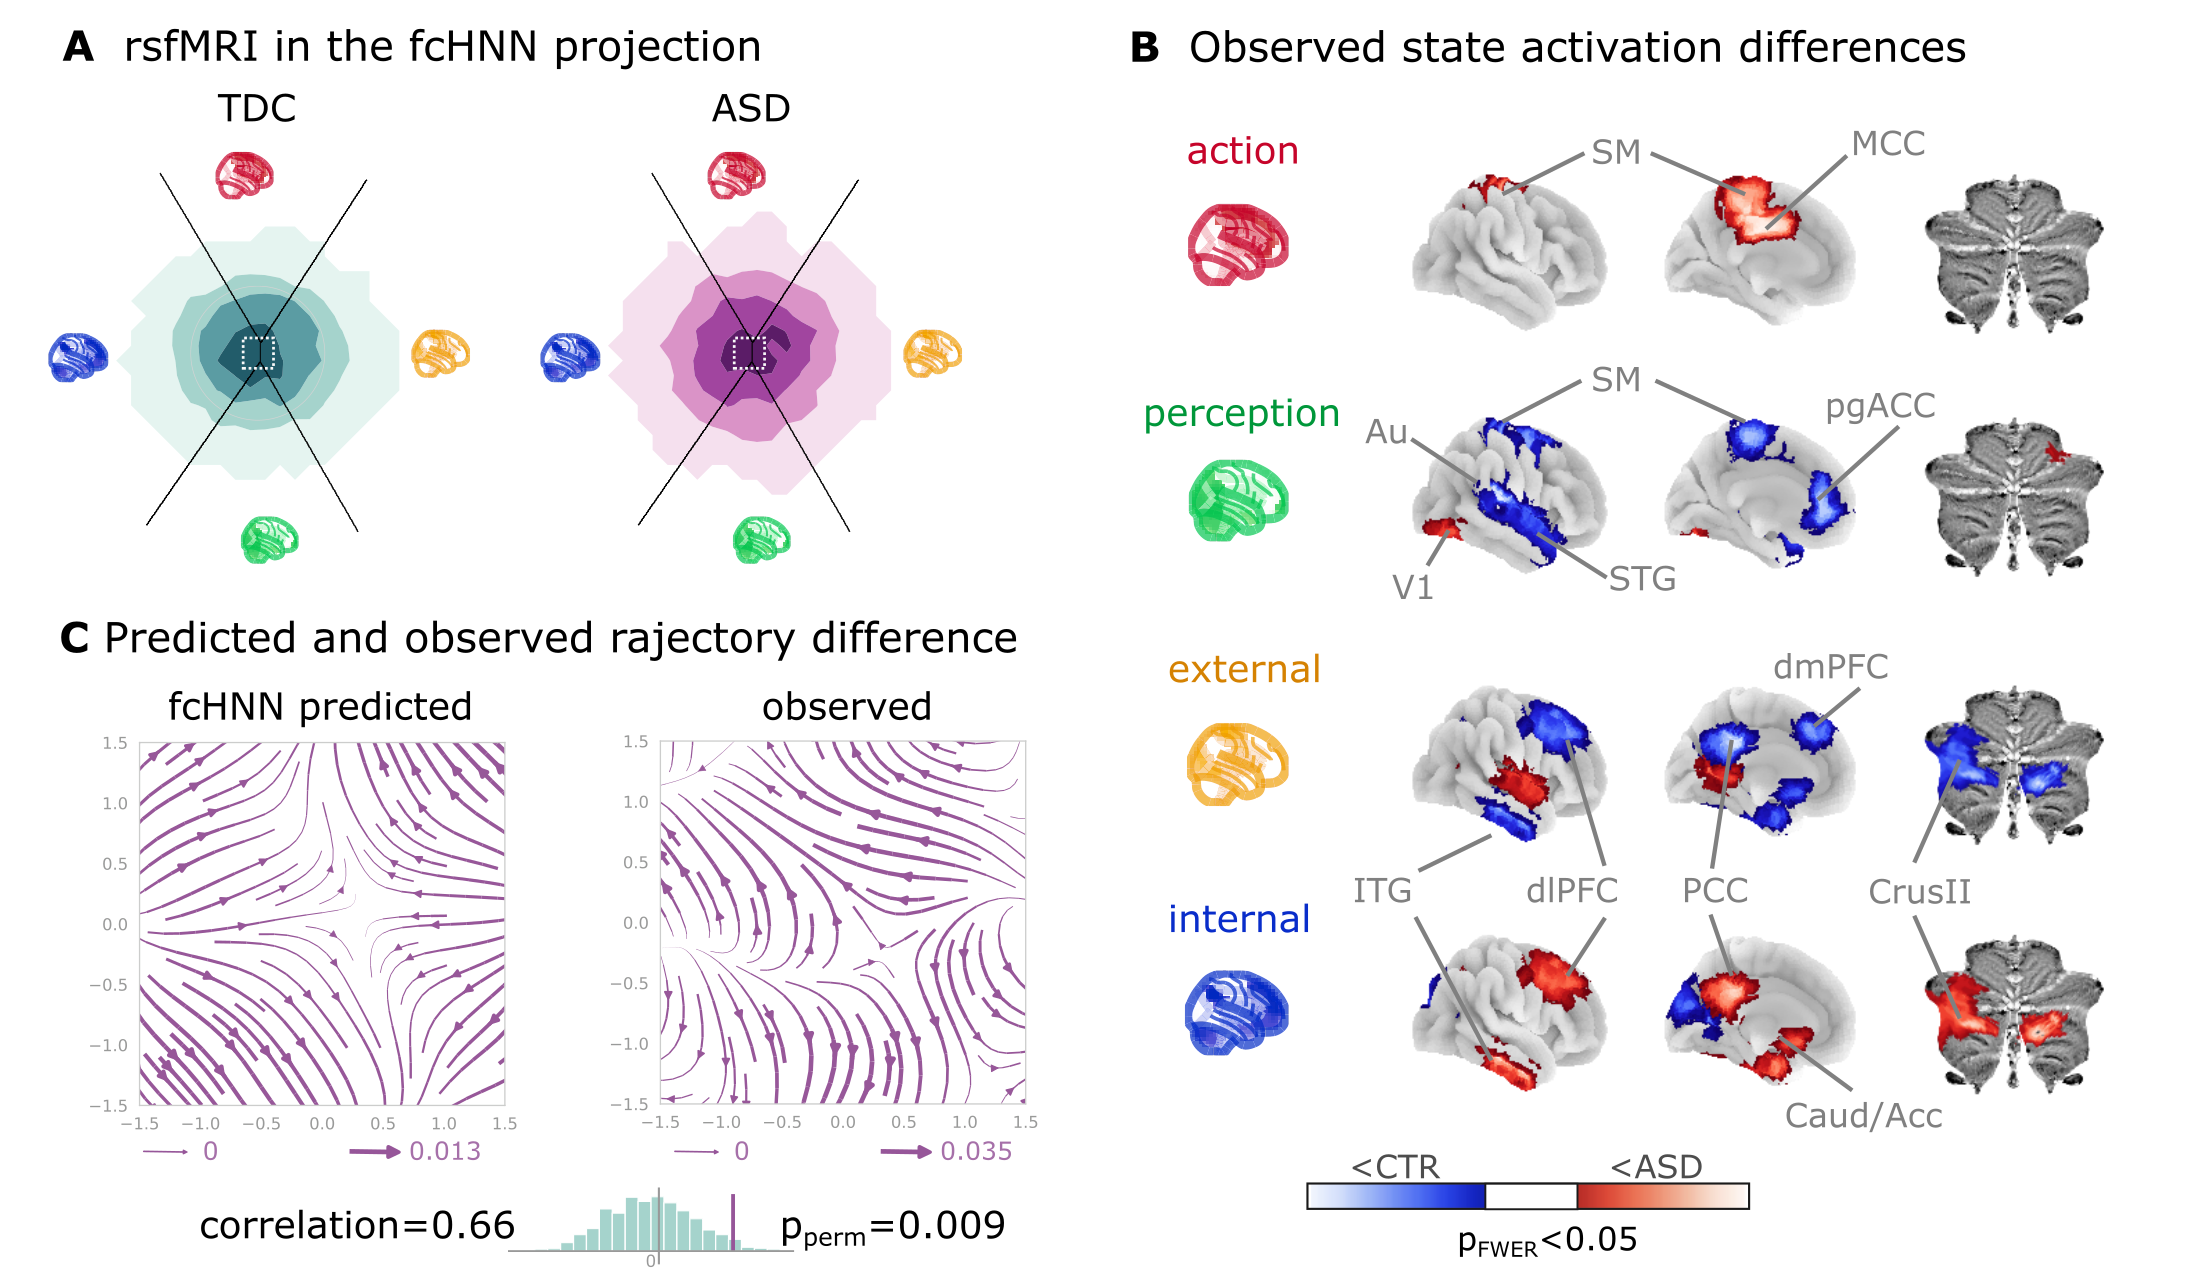
\includegraphics[width=0.7\linewidth]{files/state_analysis-62638a48ed0aff04b0227b8ef606164c.png}
\caption[]{\textbf{Connectome-based Hopfield analysis of autism spectrum disorder.} \newline

\textbf{A} The distribution of time-frames on the \acrshort{fchnn}-projection separately for \acrshort{asd} patients and typically developing control (TDC) participants. \newline

\textbf{B} We quantified attractor state activations in the Autism Brain Imaging Data Exchange datasets (Table~\ref{tab-samples}) as the
individual-level mean activation of all time-frames belonging to the same attractor state. This analysis captured alterations similar to those previously associated to \acrshort{asd}-related perceptual atypicalities (visual, auditory and somatosensory cortices) as well as atypical integration of information about the ``self'' and the ``other'' (default mode network regions). All results are corrected for multiple comparisons across brain regions and attractor states (122*4 comparisons) with Bonferroni-correction. See Table~\ref{tab-clinical-results} and Figure~\ref{si_clinical_results_table} for detailed results. \newline

\textbf{C} The comparison of data generated by \acrshort{fchnn}s initialized with \acrshort{asd} and TDC connectomes, respectively, revealed a characteristic pattern of differences in the system's dynamics, with increased pull towards (and potentially a higher separation between) the action and perception attractors and a lower tendency of trajectories going towards the internal and external attractors. \newline

\textit{\textbf{Abbreviations}: \acrshort{mcc}: mid\acrshort{dl}e cingulate cortex, \acrshort{acc}: anterior cingulate cortex, \acrshort{pg}: perigenual, \acrshort{pfc}: prefrontal cortex, \acrshort{dm}: dorsomedial, \acrshort{dl}: dorsolateral, \acrshort{stg}: superior temporal gyrus, \acrshort{itg}: inferior temporal gyrus, \acrshort{caud/acc}: caudate-accumbens,  \acrshort{sm}: sensorimotor, \acrshort{v1}: primary visual, \acrshort{a1}: primary auditory, \acrshort{sma}: supplementary motor cortex, \acrshort{asd}: autism spectrum disorder, TDC: typically developing control.}}
\label{clinical-validity}
\end{figure}

\begin{table}
\centering
\caption[]{\textbf{The top ten largest changes in average attractor-state activity between autistic and control individuals.}  Mean attractor-state activity changes are presented in the order of their absolute effect size. All p-values are based on permutation tests (shuffling the group assignment) and corrected for multiple comparisons (via Bonferroni's correction). For a comprehensive list of significant findings, see \{numref\}`Supplementary Figure \%s \textless si\_clinical\_results\_table\textgreater .}
\label{tab-clinical-results}
\begin{tabular}{p{\dimexpr 0.250\linewidth-2\tabcolsep}p{\dimexpr 0.250\linewidth-2\tabcolsep}p{\dimexpr 0.250\linewidth-2\tabcolsep}p{\dimexpr 0.250\linewidth-2\tabcolsep}}
\toprule
region & attractor & effect size & p-value \\
\hline
primary auditory cortex & perception & -0.126 & \textless 0.0001 \\
mid\acrshort{dl}e cingulate cortex & action & 0.109 & \textless 0.0001 \\
cerebellum lobule VIIb (medial part  ) & internal context & 0.104 & \textless 0.0001 \\
mediolateral sensorimotor cortex & perception & -0.099 & 0.00976 \\
precuneus & action & 0.098 & \textless 0.0001 \\
mid\acrshort{dl}e superior temporal gyrus & perception & -0.098 & \textless 0.0001 \\
frontal eye field & perception & -0.095 & \textless 0.0001 \\
dorsolateral sensorimotor cortex & perception & -0.094 & 0.00976 \\
posterior cingulate cortex & action & 0.092 & \textless 0.0001 \\
dorsolateral prefrontal cortex & external context & -0.092 & \textless 0.0001 \\
\bottomrule
\end{tabular}
\end{table}

Thus, we contrasted the characteristic trajectories derived from the \acrshort{fchnn} models of the two groups (initialized with the group-level functional connectomes). Our \acrshort{fchnn}-based flow analysis predicted that in \acrshort{asd}, there is an increased likelihood of states returning towards the mid\acrshort{dl}e (more noisy states) from the internal-external axis and an increased likelihood of states transitioning towards the extremes of the action-perception axis (Figure~\ref{clinical-validity}C). We observed a highly similar pattern in the real data (Pearson's correlation: 0.66), statistically significant after permutation testing (shuffling the group assignment, p=0.009).

\section{Discussion}

In this study, we have introduced and validated a simple and robust network-level generative computational framework that elucidates how activity propagation within the functional connectome orchestrates large-scale brain dynamics, leading to the spontaneous emergence of brain states, smooth gradients among them, and characteristic dynamic responses to perturbations.

The construct validity of our model is rooted in the activity flow principle, first introduced by \citet{cole2016activity}. The activity flow principle states that activity in a brain region can be predicted by a weighted combination of the activity of all other regions, where the weights are set to the functional connectivity of those regions to the held-out region. This principle has been shown to hold across a wide range of experimental and clinical conditions \citep{cole2016activity, ito2017cognitive, mill2022network, hearne2021activity, chen2018human}.
The proposed approach is based on the intuition that the repeated, iterative application of the activity flow equation exhibits close analogies with a type of recurrent artificial neural networks, known as Hopfield networks \citep{hopfield1982neural}.

Hopfield networks have been widely acknowledged for their relevance for brain function, including the ability to store and recall memories \citep{hopfield1982neural}, self-repair \citep{murre2003selfreparing},
a staggering robustness to noisy or corrupted inputs \citep{hertz1991introduction} (see also Figure~\ref{si_noise_robustness_weights}) and the ability to produce multistable dynamics organized by the ``gravitational pull'' of a finite number of attractor states \citep{khona2022attractor}. While many of such properties of Hopfield networks have previously been proposed as a model for micro-scale neural systems (see \cite{khona2022attractor} for a review), the proposed link between macro-scale activity propagation and Hopfield networks allows transferring the vast body of knowledge on Hopfield networks to the study of large-scale brain dynamics.

Integrating Cole's activity flow principle with the \acrshort{hnn} architecture mandates the initiation of network weights with functional connectivity values, specifically partial correlations as suggested by \citet{cole2016activity}.
Considering the functional connectome as weights of an already trained neural network distinguishes our methodology from conventional biophysical and phenomenological computational modeling strategies, which usually rely on the structural connectome to model polysynaptic connectivity \citep{cabral2017functional, deco2012anatomy, golos2015multistability, hansen2015functional}. Given the challenges of accurately modelling the structure-function coupling in the brain \citep{seguin2023brain}, such models are currently limited in terms of reconstruction accuracy, hindering translational applications.
Working with direct, functional MRI-based activity flow estimates, \acrshort{fchnn}s bypass the challenge of modelling the structural-functional coupling and provide a more direct and accurate representation of the brain's dynamic activity propagation, although at the cost of losing the ability to provide biophysical details on the underlying mechanisms.
Another advantage of the proposed model is its simplicity. While many conventional computational models rely on the optimization of a high number of free parameters, the basic form of the \acrshort{fchnn} approach comprises solely two, easily interpretable  ``hyperparameters'' (temperature and noise) and yields notably consistent outcomes across an extensive range of these parameters (Figure~\ref{si_expl_variance_energy}, Figure~\ref{si_att_state_emergence_over_beta}, Figure~\ref{si_state_occupancy_null_models}, Figure~\ref{si_pain_ghost_attractor_sim}, Figure~\ref{si_downreg_trajectory_sim}). To underscore the potency of this simplicity and stability, in the present work, we avoided any unnecessary parameter optimization, leaving a negligible chance of overwriting. It is likely, however, that extensive parameter optimization could further improve the performance of the model.

Further, the \acrshort{fchnn} approach allows us to leverage on knowledge about the underlying \acrshort{ann} architecture. Specifically, Hopfield attractor dynamics provide a mechanistic account for the emergence of large-scale canonical brain networks (Zalesky et al., 2014) ), and shed light to the origin of characteristic task-responses that are accounted by ``ghost attractors'' in the system \citep{deco2012ongoing, vohryzek2020ghost}.
As \acrshort{fchnn}s do not need to be trained to solve any explicit tasks, they are well suited to examine spontaneous brain dynamics. However, it is worth mentioning that \acrshort{fchnn}s are compatible with the neuroconnectionist approach (Doerig et al., 2021), as well.
Like any other \acrshort{ann}s, \acrshort{fchnn}s can also be further trained via established \acrshort{ann} training techniques (e.g. via the Hebbian learning rule) to ``solve'' various tasks or to match developmental dynamics or pathological alterations. In this promising future direction, the training procedure itself becomes part of the model, providing testable hypotheses about the formation, and various malformations, of brain dynamics.

Given its simplicity, it is noteworthy, how well the \acrshort{fchnn} model is able to reconstruct and predict brain dynamics under a wide range of conditions.
Our finding that the two-dimensional \acrshort{fchnn} projection can explain more variance in real resting state \acrshort{fmri} data than the first two principal components derived from the data itself may indicate that through the known noise tolerance of the underlying \acrshort{ann} architecture, \acrshort{fchnn}s are able to capture essential principles of the underlying dynamic processes even if our empirical measurements are corrupted by noise and low sampling rate.
Indeed, \acrshort{fchnn} attractor states were found to be robust to noisy weights (Figure~\ref{si_noise_robustness_weights}) and highly replicable across datasets acquired at different sites, with different scanners and imaging sequences (study 2 and 3). The observed high level of replicability allowed us to re-use the \acrshort{fchnn} model constructed with the connectome of study 1 for all subsequent analyses, without any further fine-tuning or study-specific parameter optimization.

Conceptually, the notion of a global attractor model of the brain network is not new \citep{freeman1987simulation, deco2012ongoing, vohryzek2020ghost, deco2012anatomy, golos2015multistability, hansen2015functional}.
The present work shows, however, that the brain as an attractor network necessarily `leaks its internal weights' in form of the partial correlation across the regional timeseries. This indicates that, partial correlations across neural timeseries data from different regions (i.e. functional connectivity) may be a more straightforward entry point to investigating the brain's attractor dynamics, than estimates of structural connectedness.
Thereby, the \acrshort{fchnn} approach provides a simple and interpretable way to infer and investigate the attractor states of the brain, without the need for additional assumptions about the underlying biophysical details. This is a significant advantage, as the functional connectome can be easily and non-invasively acquired in humans, while biophysical details required by other models are hard to measure or estimate accurately.
Furthermore, here we complement previous work on large-scale brain attractor dynamics, by demonstrating that the reconstructed attractor states are not solely local minima in the state-space but act as a driving force for the dynamic trajectories of brain activity. We argue that attractor-dynamics may be the main driving factor for the spatial and temporal autocorrelation structure of the brain, recently described to be predictive of network topology in relation to age, subclinical symptoms of dementia, and pharmacological manipulations with serotonergic drugs \citep{shinn2023functional}.
Nevertheless, attractor states should not be confused with the conventional notion of brain states \citep{chen2015introducing} and large-scale functional gradients \citep{margulies2016situating}. In the \acrshort{fchnn} framework, attractor states can rather be conceptualized as ``Platonic idealizations'' of brain activity, that are continuously approximated - but never reached - by the brain, resulting in re-occurring patterns (brain states) and smooth gradual transitions (large-scale gradients).

Relying on previous work, we can establish a relatively straightforward (although somewhat speculative) correspondence between attractor states and brain function, mapping brain activation on the axes of internal vs. external context \citep{golland2008data, cioli2014differences}, as well as perception vs. action \citep{fuster2004upper}.
This four-attractor architecture exhibits an appealing analogy with Friston's free energy principle \citep{friston2006free} that postulates the necessary existence of brain subsystems for active and perceptual inference and proposes that the dynamical dependencies that drive the flow of information in the brain can be represented with a hierarchically nested structure (e.g. external and internal subsystem) that may be an essential ingredient of conscious \citep{ramstead2023inner} and autonomous \citep{lee2023life} agents.

Both conceptually and in terms of analysis practices, resting and task states are often treated as separate phenomena. However, in the \acrshort{fchnn} framework, the differentiation between task and resting states is considered an artificial dichotomy.
Task-based brain activity in the \acrshort{fchnn} framework is not a mere response to external stimuli in certain brain locations but a perturbation of the brain's characteristic dynamic trajectories, with increased preference for certain locations on the energy landscape (``ghost attractors'').
In our analyses, the \acrshort{fchnn} approach captured and predicted participant-level activity changes induced by pain and its self-regulation and gave a mechanistic account for how relatively small activity changes in a single region (NAcc) may result in a significantly altered pain experience.
Our control-signal analysis is different from, but compatible with, linear network control theory-based (Gu et al., 2015) approaches. Combining network control theory with the \acrshort{fchnn} approach could provide a powerful framework for understanding the effects of various tasks, conditions and interventions (e.g. brain stimulation) on brain dynamics.

Brain dynamics can not only be perturbed by task or other types of experimental or naturalistic interventions, but also by pathological alterations. Here we provide an initial demonstration (study 7) of how \acrshort{fchnn}-based analyses can characterize and predict altered brain dynamics in autism spectrum disorder (\acrshort{asd}). The observed \acrshort{asd}-associated changes in brain dynamics are indicative of a reduced ability to flexibly switch between perception and internal representations, corroborating previous findings that in \acrshort{asd}, sensory-driven connectivity transitions do not converge to transmodal areas \citep{hong2019atypical}. Such findings are in line with previous reports of a reduced influence of context on the interpretation of incoming sensory information in \acrshort{asd} (e.g. the violation of Weber's law) \citep{hadad2019perception}.

Our findings open up a series of exciting opportunities for the better understanding of brain function in health and disease.
First, the 2-dimensional \acrshort{fchnn} projection offers a simple framework not only for the visualization, but also for the \textit{interpretation}, of brain activity patterns, as it conceptualizes changes related to various behavioral or clinical states or traits as a shift in brain dynamics in relation to brain attractor states.
Second, \acrshort{fchnn} analyses may provide insights into the causes of changes in brain dynamics, by for instance, identifying the regions or connections that act as an ``Achilles heel'' in generating such changes. Such control analyses could, for instance, aid the differentiation of primary causes and secondary effects of activity or connectivity changes in various clinical conditions.
Third, the \acrshort{fchnn} approach can provide testable predictions about the effects of pharmacological interventions as well as non-invasive brain stimulation (e.g. transcranial magnetic or direct current stimulation, focused ultrasound, etc.) and neurofeedback. Obtaining the optimal stimulation or treatment target within the \acrshort{fchnn} framework (e.g. by means of network control theory \citep{liu2011controllability}) is one of the most promising future directions with the potential to significantly advance the development of novel, personalized treatment approaches.

The proposed approach is not without limitations. First, the \acrshort{fchnn} model is obviously a simplification of the brain's dynamics, and it does not aim to explain the brain's ability to perform certain computations, brain regions' ability to perform certain functions or biophysical details underlying (altered) polysynaptic connections. Nevertheless, our approach showcases that many characteristics of brain dynamics, like multistability, temporal autocorrelations, states and gradients, can be explained, and predicted, by a very simple nonlinear phenomenological model.
Second, our model assumes a stationary connectome, which seems to contradict notions of dynamic connectivity. However, with realistically changing control signals, our model can easily reconstruct dynamic connectivity changes, which still stem from an underlying, stationary functional connectivity structure. This is in line with the notion of ``latent functional connectivity''; and intrinsic brain network architecture built up from connectivity properties that are persistent across brain states \cite{McCormick_2022}.
In this initial work, we presented the simplest possible implementation of the \acrshort{fchnn} concept. It is clear that the presented analyses exploit only a small proportion of the richness of the full state-space dynamics reconstructed by the \acrshort{fchnn} model.
There are many potential ways to further improve the utility of the \acrshort{fchnn} approach. Increasing the number of reconstructed attractor states (by increasing the temperature parameter), investigating higher-dimensional dynamics, fine-tuning the hyperparameters, testing the effect of different initializations and perturbations are all important direction for future work, with the potential to further improve the model's accuracy and usefulness.

\section{Conclusion}

To conclude, here we have proposed a lightweight, high-level computational framework that accurately captures and predicts brain dynamics under a wide range of conditions, including resting states, task-induced activity changes and brain disorders. The framework models large-scale activity flow in the brain with a recurrent artificial neural network architecture that, instead of being trained to solve specific tasks or mimic certain dynamics, is simply initialized with the empirical functional connectome. The framework identifies neurobiologically meaningful attractor states and provides a model for how these restrict brain dynamics.
The proposed model establishes a conceptual link between connectivity and activity, provides a mechanistic account for the emergence of brain states, gradients and temporal autocorrelation structure and offers a simple, robust, and highly interpretable computational alternative to conventional descriptive approaches to investigating brain function. The generative nature of our proposed model opens up a wealth of opportunities for future research, including predicting the effect, and understanding the mechanistic bases, of various interventions; thereby paving the way for designing novel treatment approaches.

% +++ {"part": "acknowledgements"}

\section{Acknowledgements}

The work was supported by the Deutsche Forschungsgemeinschaft (DFG, German Research Foundation; projects `TRR289 - Treatment Expectation', ID 422744262 and `SFB1280 - Extinction Learning', ID 316803389) and by IBS-R015-D1 (Institute for Basic Science; C.W.-W.).

% +++

% +++ {"part": "data-availability"}

\section{Analysis source code}

\href{https://github.com/pni-lab/connattractor}{https://github.com/pni-lab/connattractor}

\section{Project website}

\href{https://pni-lab.github.io/connattractor/}{https://pni-lab.github.io/connattractor/}

\section{Data availability}

Study 1, 2 and 4 is available at \href{http://openneuro.org}{openneuro.org} (ds002608, ds002608, ds000140). Data for study 3 is available upon request. Data for study 5-6 is available at the github page of the project: \href{https://github.com/pni-lab/connattractor}{https://github.com/pni-lab/connattractor}. Study 7 is available at https://fcon\_1000.projects.nitrc.org/indi/abide/, preprocessed data is available at \href{http://preprocessed-connectomes-project.org/}{http://preprocessed-connectomes-project.org/}.

% +++
%%%%%%%%%%%%%%%%%%%%%%%%%%%%%%%%%%%%%%%%%%%%%%%%%%
%%%%%%%%%%%%%%  acronyms & glossary  %%%%%%%%%%%%%
\printglossaries
%%%%%%%%%%%%%%%%%%%%%%%%%%%%%%%%%%%%%%%%%%%%%%%%%%




\bibliographystyle{unsrtnat}
\bibliography{main.bib}

\end{document}
